\documentclass[a4paper, 10pt, twoside]{article}

%=============== LIBRERIA ===============
\usepackage{lmodern}
\usepackage{fontspec}
\usepackage[utf8]{inputenc}
\usepackage[italian]{babel}

% gestione dei font e gli spazi tra le righe
\usepackage{setspace}
\usepackage{setspace}
\singlespace 

% gestione tabelle
\usepackage{tabularray}

% gestione dei margini del pdf
\usepackage{geometry}
\geometry{a4paper, lmargin=2cm, rmargin=2cm, tmargin=2cm, bmargin=2cm}

 % libreria per riferimenti esterni ed interni
\usepackage{hyperref}
\hypersetup{
    colorlinks,
    citecolor=black,
    filecolor=black,
    linkcolor=black,
    urlcolor=black
}

% libreria per l'indici
\usepackage{makeidx}

% gestione grafica e figure
\usepackage{graphicx}
\usepackage{wrapfig}
% \usepackage[inkscapeformat=png]{svg}  % richiede inkscape: si usa il PNG in img/

% scrivere in colonne diverse
\usepackage{multicol}
\setlength{\columnsep}{0.5cm}

% RIGA
\newcommand{\HRule}{\noindent\rule{\linewidth}{0.5mm}}

% RIGA COLORATA
\newcommand{\ColorHRule}[1]{\noindent\textcolor{#1}{\rule{\linewidth}{0.5mm}\\}}

% CREAZIONE COVERPAGE
\newcommand{\Cover}[2]{
\begin{titlepage}
    \begin{center}
      % logo
      
\includegraphics[width=0.5\textwidth]{img/logo_unina.png}\\[1cm]
  
      \textsc{\Large A.A 2026/27 \\ CdS: Fisica}\\[2cm]
  
      \HRule \\[0.4cm]
      {\large \bfseries #1 \\ prof: #2 \\[0.4cm]}
      \HRule \\[3cm]
  
      \large\textbf{Studente:} Gianmarco Davini \\ Dipartimento di Fisica Ettore Pancini \\ Università Federico II\\[3cm]
    \end{center}
\end{titlepage}

\tableofcontents
\newpage
}

% librerie matematica
\usepackage{siunitx} % fornisce dei typeset per i numeri e le unita di misura
\usepackage{amssymb}
\usepackage{amsthm}

\usepackage{amsfonts}

% emoji
%\usepackage{fourier}
% \usepackage{emoji}  % richiede LuaLaTeX + font emoji a colori

% creazione dei Toast message
\usepackage[many]{tcolorbox}

% definizione di nuovi colori
\usepackage{xcolor}

% SIMBOLO MATEMATICO ESISTE ED E' UNICO
\newcommand{\existsone}{\exists !}

% INSIEMI MATEMATICI
\newcommand{\R}{\mathbb{R}}
\newcommand{\N}{\mathbb{N}}
\newcommand{\Z}{\mathbb{Z}}
\newcommand{\C}{\mathbb{C}}

% DEFINIZIONE
\definecolor{myred}{RGB}{191,101,127}
\definecolor{mygreen}{RGB}{0,168,107}

\definecolor{myblue}{RGB}{0,127,255}
\definecolor{myblue2}{RGB}{36,84,255}

\definecolor{myyellow}{RGB}{255,191,0}
\definecolor{mygray}{RGB}{83,104,120}

% BOX VUOTI
\newtcolorbox{empty_green}{enhanced, toprule=0pt, bottomrule=0pt, rightrule=0pt, leftrule=3pt, arc=0mm, skin=enhancedlast jigsaw, sharp corners,
colframe=mygreen, colbacktitle=mygreen}

\newtcolorbox{empty_red}{enhanced, toprule=0pt, bottomrule=0pt, rightrule=0pt, leftrule=3pt, arc=0mm, skin=enhancedlast jigsaw, sharp corners,
colframe=myred, colbacktitle=myred}

\newtcolorbox{empty_blue}{enhanced, toprule=0pt, bottomrule=0pt, rightrule=0pt, leftrule=3pt, arc=0mm, skin=enhancedlast jigsaw, sharp corners,
colframe=myblue, colbacktitle=myblue}

\newtcolorbox{empty_yellow}{enhanced, toprule=0pt, bottomrule=0pt, rightrule=0pt, leftrule=3pt, arc=0mm, skin=enhancedlast jigsaw, sharp corners,
colframe=myyellow, colbacktitle=myyellow}


\newcommand{\BoxRed}[3]{
    \begin{empty_red}
        \textcolor{myred}{\textbf{#1} \textbf{#2}}\\
        \noindent #3
    \end{empty_red}
}

\newcommand{\BoxGreen}[3]{
    \begin{empty_green}
        \textcolor{mygreen}{\textbf{#1} \textbf{#2}}\\
        \noindent #3
    \end{empty_green}
}

\newcommand{\BoxBlue}[3]{
    \begin{empty_blue}
        \textcolor{myblue}{\textbf{#1} \textbf{#2}}\\
        \noindent #3
    \end{empty_blue}
}

\newcommand{\Attenzione}[1]{
    \begin{empty_yellow}
        \textbf{\Large !}\enspace #1
    \end{empty_yellow}
}

\newcommand{\Definizione}[2]{
    \begin{empty_green}
         \textcolor{mygreen}{\textbf{Definizione (#1)}}\\
        \noindent #2
    \end{empty_green}
}

\newcommand{\Teorema}[2]{
    \begin{empty_red}
        \textcolor{myred}{\textbf{Teorema (#1)}}\\
        \noindent #2
    \end{empty_red}
}

\newcommand{\Dimostrazione}[1]{
    \begin{empty_blue}
        \textcolor{myblue}{\textbf{Dimostrazione}}\\
        \noindent \textcolor{myblue}{#1}
    \end{empty_blue}
}

% ---- pacchetti aggiuntivi richiesti dagli argomenti ----
\usepackage{amsmath}    % aligned, dfrac, xrightarrow, ...
\usepackage{float}      % per [H] nelle figure
\usepackage{needspace}  % evita titoli orfani a fine pagina
\newcommand{\Xconv}{\overline{\underline{X}}} % insieme di convergenza
\begin{document}

\Cover{Analisi Matematica II}{Nunzia Gavitone}

% ---------------- Lezione 1 ----------------
% =====================================================================
%  Successioni di funzioni -- capitolo 1
% =====================================================================

\section{Successioni di funzioni}

\subsection{Motivazione: da Taylor alle serie di funzioni}

Sia $I \subseteq \mathbb{R}$ un intervallo, $x_0 \in I$ e $f \in C^\infty(I)$.
Poiché $f$ è derivabile quante volte si vuole, per \emph{ogni} $n \in \mathbb{N}$
possiamo scrivere il polinomio di Taylor di ordine $n$ centrato in $x_0$:
\[
\begin{aligned}
  P_n(x) &= \sum_{k=0}^{n} \frac{f^{(k)}(x_0)}{k!}\,(x-x_0)^k \\
         &= f(x_0) + f'(x_0)(x-x_0) + \frac{f''(x_0)}{2!}(x-x_0)^2 + \dots
            + \frac{f^{(n)}(x_0)}{n!}(x-x_0)^n .
\end{aligned}
\]

In Analisi~I lo abbiamo usato nella \textbf{formula di Taylor con resto di Peano}:
\[
  f(x) \;=\; P_n(x) + o\big((x-x_0)^n\big) \qquad \text{per } x \to x_0 .
\]
Qui $n$ è \emph{fissato} e l'informazione è solo \emph{locale}: vale vicino a $x_0$.

Ora ci chiediamo cosa succede se lasciamo crescere $n$ senza limite, cioè se ha
senso scrivere
\[
  f(x) \;=\; \sum_{k=0}^{\infty} \frac{f^{(k)}(x_0)}{k!}\,(x-x_0)^k
  \;=\; a_0 + a_1 (x-x_0) + a_2 (x-x_0)^2 + \dots ,
  \qquad a_k = \frac{f^{(k)}(x_0)}{k!} .
\]
Il membro destro è una \textbf{somma infinita di funzioni}, cioè una
\textbf{serie di funzioni}. Come per le serie numeriche, la sua somma va intesa
come limite delle somme parziali:
\[
  \sum_{k=0}^{\infty} \frac{f^{(k)}(x_0)}{k!}\,(x-x_0)^k
  \;:=\; \lim_{n \to +\infty} P_n(x) .
\]
Le somme parziali $P_0, P_1, P_2, \dots$ però non sono numeri, sono
\emph{funzioni}. Per dare senso a questo limite serve prima capire cosa vuol dire
che una \textbf{successione di funzioni} converge: è l'argomento di questo capitolo.

\BoxBlue{Attenzione}{}{%
  $f \in C^\infty$ garantisce che la serie di Taylor si possa \emph{scrivere},
  ma \textbf{non} che converga a $f$. Ad esempio
  \[
    f(x) =
    \begin{cases}
      e^{-1/x^2} & x \neq 0 \\[2pt]
      0          & x = 0
    \end{cases}
  \]
  è $C^\infty(\mathbb{R})$ con $f^{(k)}(0) = 0$ per ogni $k$: la sua serie di
  Taylor in $0$ è identicamente nulla, mentre $f(x) > 0$ per $x \neq 0$.
  Le funzioni che coincidono con la propria serie di Taylor si dicono
  \textbf{analitiche}.
}

\subsection{Definizione}

\BoxBlue{Richiamo (successione numerica)}{}{%
  Una successione numerica è una legge che a ogni $n \in \mathbb{N}$ associa
  un numero reale:
  \[
    n \longmapsto a_n \in \mathbb{R} .
  \]
}

\BoxGreen{Definizione (successione di funzioni)}{}{%
  Sia $I \subseteq \mathbb{R}$. Una \textbf{successione di funzioni} definite in
  $I$ è una legge che a ogni $n \in \mathbb{N}$ associa una funzione
  \[
    n \longmapsto f_n : I \to \mathbb{R} .
  \]
  Si indica con $(f_n)_{n \in \mathbb{N}}$ o semplicemente $(f_n)$.
}

L'insieme di definizione $I$ va \textbf{sempre} indicato: come vedremo, il
comportamento della successione dipende fortemente da $I$.

\BoxBlue{Osservazione}{}{%
  L'espressione $f_n(x)$ dipende da \textbf{due variabili indipendenti},
  $n \in \mathbb{N}$ e $x \in I$:
  \begin{itemize}
    \item fissato $n$, si ottiene una \emph{funzione} $x \mapsto f_n(x)$;
    \item fissato $x \in I$, si ottiene una \emph{successione numerica}
          $n \mapsto f_n(x)$.
  \end{itemize}
  Il secondo punto è quello che ci permetterà di riusare quanto sappiamo sui
  limiti di successioni numeriche.
}

\paragraph{Esempio 1.} Consideriamo
\[
  f_n(x) = \frac{x}{n}, \qquad x \in \mathbb{R} .
\]

\emph{Fissando $n$} otteniamo le funzioni
\[
  f_1(x) = x, \qquad f_2(x) = \frac{x}{2}, \qquad f_3(x) = \frac{x}{3},
  \qquad \dots
\]
cioè rette per l'origine con pendenza $1/n$.

\emph{Fissando $x$} otteniamo successioni numeriche:
\[
  x = 1: \quad f_n(1) = \frac{1}{n},
  \qquad\qquad
  x = 2: \quad f_n(2) = \frac{2}{n},
  \qquad\qquad
  x \text{ generico}: \quad f_n(x) = \frac{x}{n} .
\]
Per ogni $x$ fissato vale $f_n(x) \to 0$: nella prossima sezione vedremo come
questo si legge sul grafico e come formalizzarlo.

% ---------------------------------------------------------------------
\subsection{Rappresentazione grafica}

Disegnando sullo stesso piano i grafici di $f_1, f_2, f_3, \dots$ otteniamo un
\emph{fascio di grafici}. Per $f_n(x) = x/n$ sono rette per l'origine che, al
crescere di $n$, si adagiano sull'asse $x$.

\begin{figure}[H]
\centering
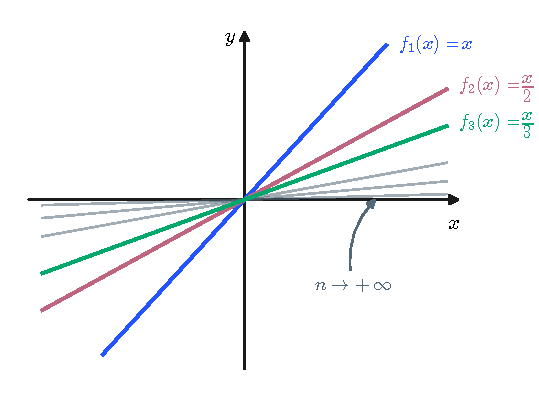
\includegraphics[width=0.78\textwidth]{immagini/succ_fascio_rette}
\caption{Le funzioni $f_n(x) = x/n$: al crescere di $n$ le rette si schiacciano
sull'asse $x$.}
\end{figure}

Il grafico suggerisce che le $f_n$ ``tendono'' alla funzione costante
\[
  f(x) = 0 .
\]
Dobbiamo dare un significato preciso a questa affermazione.

% ---------------------------------------------------------------------
\subsection{Convergenza puntuale}

\BoxBlue{Richiamo (limite di una successione numerica)}{}{%
  \[
    \lim_{n \to +\infty} a_n = \ell \in \mathbb{R}
    \iff
    \forall \varepsilon > 0 \;\; \exists\, \nu_\varepsilon \in \mathbb{N} :
    \;\; |a_n - \ell| < \varepsilon \quad \forall n > \nu_\varepsilon .
  \]
}

L'idea più naturale è fissare $x \in I$ e applicare questa definizione alla
successione numerica $n \mapsto f_n(x)$.

\BoxGreen{Definizione (convergenza puntuale)}{}{%
  Siano $f_n : I \to \mathbb{R}$ e $f : I \to \mathbb{R}$. Diciamo che $(f_n)$
  \textbf{converge puntualmente} a $f$ in $I$ se
  \[
    \lim_{n \to +\infty} f_n(x) = f(x) \qquad \forall x \in I .
  \]
  La funzione $f$ si chiama \textbf{limite puntuale} della successione.
}

Esplicitando il limite, la definizione diventa
\[
  \forall x \in I \;\; \forall \varepsilon > 0 \;\; \exists\, \nu_{\varepsilon,x} \in \mathbb{N} :
  \;\; |f_n(x) - f(x)| < \varepsilon \quad \forall n > \nu_{\varepsilon,x} .
\]
L'indice $\nu_{\varepsilon,x}$ dipende \textbf{sia da $\varepsilon$ sia da $x$}:
in punti diversi la successione può avvicinarsi al limite con velocità molto
diverse. Questo dettaglio sarà il cuore della sezione~\ref{sec:unif}.

\paragraph{Notazione.} Si scrive indifferentemente
\[
  \lim_{n \to +\infty} f_n(x) = f(x) \;\; \forall x \in I
  \qquad \text{oppure} \qquad
  f_n \xrightarrow{\;p\;} f \;\; \text{in } I .
\]
Il limite è sempre fatto per $n \to +\infty$, con $x$ fissato: la variabile $x$
\emph{non} va da nessuna parte.

% ---------------------------------------------------------------------
\subsection{Calcolo del limite puntuale: esempi}

Il metodo è sempre lo stesso: si fissa $x$, si calcola il limite in $n$ e si
controlla se esistono valori di $x$ per cui il calcolo cambia.

\paragraph{Esempio 1 (ripreso).}
\[
  f_n(x) = \frac{x}{n}, \qquad x \in \mathbb{R}.
\]
Per ogni $x$ fissato il numeratore è costante e il denominatore diverge, quindi
\[
  f_n \xrightarrow{\;p\;} f \equiv 0 \quad \text{in } \mathbb{R} .
\]

\paragraph{Esempio 2.}
\[
  f_n(x) = \frac{n + x}{n + (-1)^n \sqrt{n}}, \qquad x \in \mathbb{R}, \;\; n \ge 2
\]
(per $n = 1$ il denominatore si annulla). Dividendo numeratore e denominatore
per $n$:
\[
  f_n(x) = \frac{1 + \dfrac{x}{n}}{1 + \dfrac{(-1)^n}{\sqrt{n}}}
  \;\longrightarrow\; \frac{1 + 0}{1 + 0} = 1 ,
\]
quindi
\[
  f_n \xrightarrow{\;p\;} f \equiv 1 \quad \text{in } \mathbb{R} .
\]

\paragraph{Esempio 3.}
\[
  f_n(x) = \frac{n}{n^2 x + 2n - 1} .
\]
Qui il termine dominante del denominatore è $n^2 x$, che però \textbf{sparisce
se $x = 0$}: i due casi vanno trattati separatamente.
\begin{itemize}
  \item Se $x \neq 0$, dividendo per $n$:
  \[
    f_n(x) = \frac{1}{n x + 2 - \dfrac{1}{n}} \longrightarrow 0 ,
    \qquad \text{perché } |n x| \to +\infty .
  \]
  \item Se $x = 0$:
  \[
    f_n(0) = \frac{n}{2n - 1} \longrightarrow \frac{1}{2} .
  \]
\end{itemize}
Quindi
\[
  f_n \xrightarrow{\;p\;} f(x) =
  \begin{cases}
    0           & x \neq 0 \\[2pt]
    \dfrac{1}{2} & x = 0
  \end{cases}
  \qquad \text{in } \mathbb{R} .
\]

\BoxBlue{Osservazione}{}{%
  $f_n$ non è definita dove $n^2 x + 2n - 1 = 0$. Per $x$ fissato, però, questa
  è un'equazione di secondo grado in $n$ e ha al più due soluzioni: da un certo
  $n$ in poi $f_n(x)$ è definita e il limite ha senso.

  Morale: bisogna sempre guardare \emph{come interagiscono} $x$ e $n$. I valori
  di $x$ che annullano il termine dominante vanno studiati a parte.
}

\paragraph{Esempio 4.}
\[
  f_n(x) = x^n, \qquad x \in [0,1] .
\]
Per $0 \le x < 1$ si ha $x^n \to 0$, mentre per $x = 1$ si ha $1^n = 1$. Quindi
\[
  f_n \xrightarrow{\;p\;} f(x) =
  \begin{cases}
    0 & 0 \le x < 1 \\[2pt]
    1 & x = 1
  \end{cases}
  \qquad \text{in } [0,1] .
\]

\begin{figure}[H]
\centering
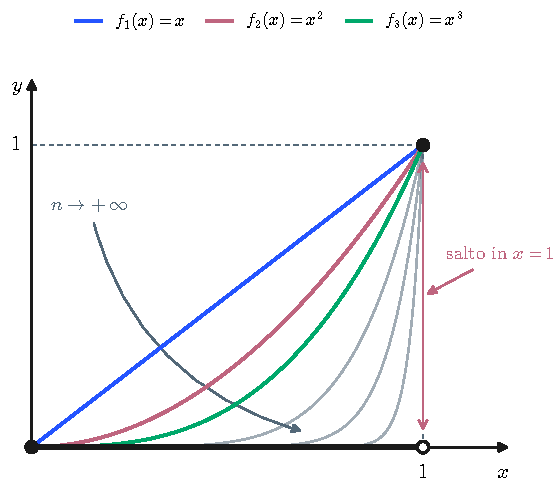
\includegraphics[width=0.62\textwidth]{immagini/succ_xn_puntuale}
\caption{$f_n(x) = x^n$ su $[0,1]$. In nero il limite puntuale: vale $0$ su
$[0,1[$ e salta a $1$ in $x = 1$.}
\end{figure}

\paragraph{Esempio 5.}
\[
  f_n(x) = x^{1/n} = \sqrt[n]{x}, \qquad x \in [0,1] .
\]
Per $x \in \,]0,1]$ si ha $x^{1/n} \to x^0 = 1$, mentre $f_n(0) = 0$ per ogni $n$.
Quindi
\[
  f_n \xrightarrow{\;p\;} f(x) =
  \begin{cases}
    0 & x = 0 \\[2pt]
    1 & 0 < x \le 1
  \end{cases}
  \qquad \text{in } [0,1] .
\]

\begin{figure}[H]
\centering
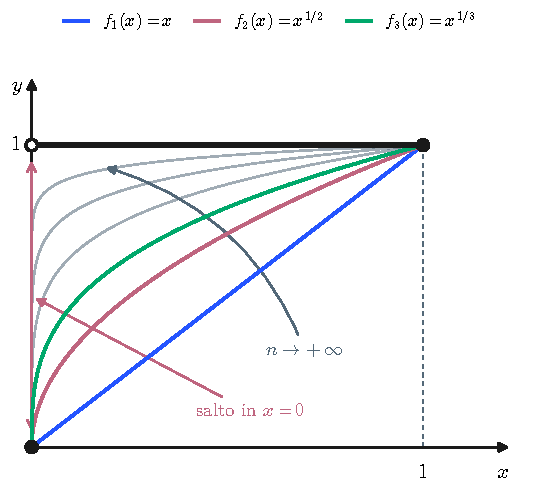
\includegraphics[width=0.62\textwidth]{immagini/succ_x1n_puntuale}
\caption{$f_n(x) = x^{1/n}$ su $[0,1]$. In nero il limite puntuale: vale $1$ su
$]0,1]$ e salta a $0$ in $x = 0$.}
\end{figure}

% ---------------------------------------------------------------------
\subsection{I limiti della convergenza puntuale}

\BoxBlue{Osservazione}{}{%
  Negli esempi 4 e 5 le $f_n$ sono tutte continue (le $x^n$ sono addirittura
  $C^\infty$), ma il limite puntuale \textbf{non è nemmeno continuo}.
  La convergenza puntuale, quindi, non conserva la continuità, e a maggior
  ragione non conserva la derivabilità.
}

Questo è un problema serio per il nostro obiettivo: vogliamo scrivere funzioni
come limiti di polinomi e continuare a lavorarci sopra (derivarle, integrarle).
Serve una \textbf{nozione di convergenza più forte}, che trasmetta al limite le
buone proprietà delle $f_n$.

Mettiamo a confronto i tre esempi principali visti finora.

\begin{figure}[H]
\centering
\begin{minipage}{0.32\textwidth}\centering
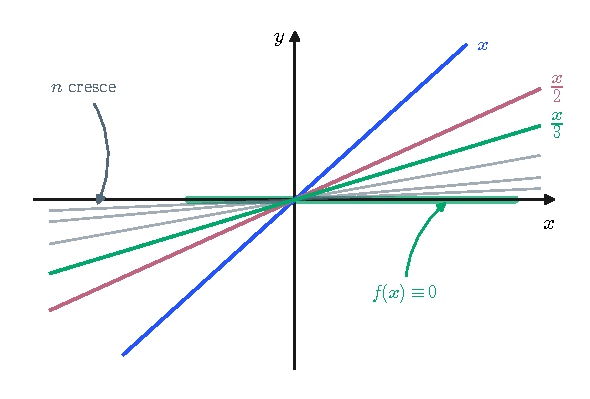
\includegraphics[width=\linewidth]{immagini/unif_fascio_rette}\\[2pt]
{\small $\dfrac{x}{n}$ in $\mathbb{R}$: limite $f \equiv 0$, continuo}
\end{minipage}\hfill
\begin{minipage}{0.32\textwidth}\centering
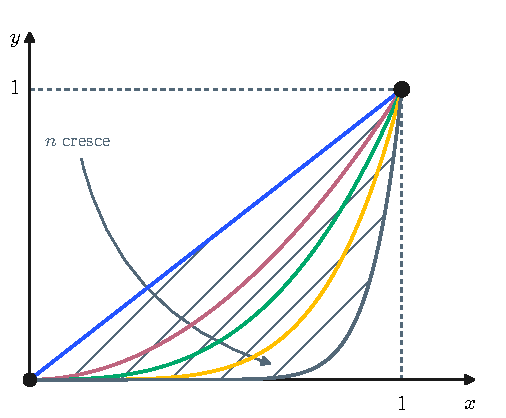
\includegraphics[width=\linewidth]{immagini/unif_xn_tratteggio}\\[2pt]
{\small $x^n$ in $[0,1]$: limite discontinuo in $x = 1$}
\end{minipage}\hfill
\begin{minipage}{0.32\textwidth}\centering
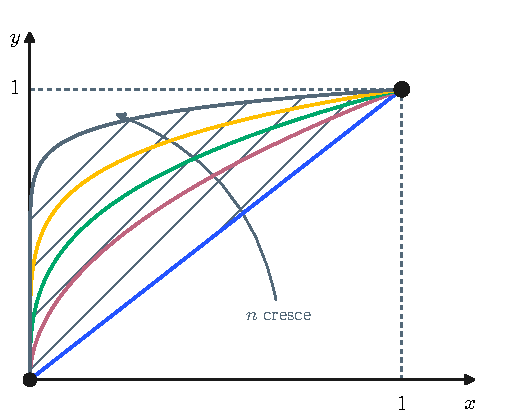
\includegraphics[width=\linewidth]{immagini/unif_x1n_tratteggio}\\[2pt]
{\small $x^{1/n}$ in $[0,1]$: limite discontinuo in $x = 0$}
\end{minipage}
\caption{I tre esempi a confronto. In nero, il limite puntuale.}
\end{figure}

Nel primo caso il limite è continuo, negli altri due no. Vedremo però che anche
nel primo caso la convergenza ha un difetto: le rette si avvicinano all'asse $x$
sempre più lentamente man mano che $|x|$ cresce.

% ---------------------------------------------------------------------
\subsection{Convergenza uniforme}\label{sec:unif}

Il difetto della convergenza puntuale sta nel fatto che $\nu_{\varepsilon,x}$
dipende da $x$. Negli esempi 4 e 5, più ci si avvicina al punto di salto, più
$n$ deve essere grande per avere $|f_n(x) - f(x)| < \varepsilon$. Chiediamo
allora che uno stesso indice funzioni \emph{per tutti} gli $x$.

\BoxGreen{Definizione (convergenza uniforme)}{}{%
  Siano $f_n : I \to \mathbb{R}$ e $f : I \to \mathbb{R}$. Diciamo che $(f_n)$
  \textbf{converge uniformemente} a $f$ in $I$, e scriviamo
  $f_n \rightrightarrows f$ in $I$, se
  \[
    \forall \varepsilon > 0 \;\; \exists\, \nu_\varepsilon \in \mathbb{N} :
    \;\; |f_n(x) - f(x)| < \varepsilon \quad \forall n > \nu_\varepsilon, \;\; \forall x \in I .
  \]
}

Conviene confrontare le due definizioni: cambia solo \textbf{la posizione di
``$\forall x$''}.
\[
\begin{aligned}
  \text{puntuale:} \quad & \forall x \in I \;\; \forall \varepsilon > 0 \;\; \exists\, \nu_{\varepsilon,x} : \;\; |f_n(x) - f(x)| < \varepsilon \;\; \forall n > \nu_{\varepsilon,x} \\[4pt]
  \text{uniforme:} \quad & \forall \varepsilon > 0 \;\; \exists\, \nu_{\varepsilon} : \;\; |f_n(x) - f(x)| < \varepsilon \;\; \forall n > \nu_{\varepsilon}, \;\; \forall x \in I
\end{aligned}
\]
Nel primo caso $x$ viene scelto \emph{prima} di $\nu$, che quindi può dipenderne;
nel secondo $\nu$ viene scelto prima di $x$ e deve andare bene per tutti.

\paragraph{Interpretazione grafica.} La condizione
$|f_n(x) - f(x)| < \varepsilon$ per ogni $x \in I$ significa
\[
  f(x) - \varepsilon < f_n(x) < f(x) + \varepsilon \qquad \forall x \in I ,
\]
cioè il grafico di $f_n$ sta tutto dentro il ``tubo'' di raggio $\varepsilon$
attorno al grafico di $f$. La convergenza è uniforme se, comunque si scelga lo
spessore $\varepsilon$ del tubo, da un certo indice in poi \emph{tutti} i grafici
delle $f_n$ ci stanno dentro.

\begin{figure}[H]
\centering
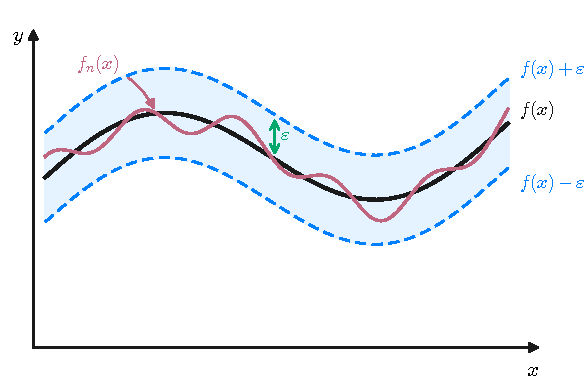
\includegraphics[width=0.88\textwidth]{immagini/tubo_epsilon}
\caption{Per $n > \nu_\varepsilon$ il grafico di ogni $f_n$ è contenuto nel tubo
di raggio $\varepsilon$ attorno a $f$.}
\end{figure}

% ---------------------------------------------------------------------
\subsection{Caratterizzazione con l'estremo superiore}

Verificare la definizione ``a mano'' è scomodo. Si usa quasi sempre questa
forma equivalente. Per ogni $n$ poniamo
\[
  M_n := \sup_{x \in I} |f_n(x) - f(x)| \;\in [0, +\infty] .
\]
Fissato $n$, $M_n$ è un \emph{numero}: la massima distanza verticale tra i
grafici di $f_n$ e $f$. Quindi $(M_n)$ è una \emph{successione numerica}.

\BoxGreen{Teorema (caratterizzazione della convergenza uniforme)}{}{%
  \[
    f_n \rightrightarrows f \;\; \text{in } I
    \iff
    \lim_{n \to +\infty} \, \sup_{x \in I} |f_n(x) - f(x)| = 0 .
  \]
}

\noindent\textit{Dimostrazione.}
($\Rightarrow$) Fissato $\varepsilon > 0$, per $n > \nu_\varepsilon$ vale
$|f_n(x) - f(x)| < \varepsilon$ per ogni $x \in I$. Passando all'estremo
superiore
\[
  M_n \le \varepsilon \qquad \forall n > \nu_\varepsilon ,
\]
(il $<$ diventa $\le$, ma per l'arbitrarietà di $\varepsilon$ non cambia nulla),
quindi $M_n \to 0$.

($\Leftarrow$) Se $M_n \to 0$, fissato $\varepsilon > 0$ esiste
$\nu_\varepsilon$ tale che $M_n < \varepsilon$ per $n > \nu_\varepsilon$. Allora,
per ogni $x \in I$,
\[
  |f_n(x) - f(x)| \le M_n < \varepsilon \qquad \forall n > \nu_\varepsilon . \qquad \square
\]

\paragraph{Ricetta operativa.}
\begin{enumerate}
  \item Si calcola il limite puntuale $f$.
  \item Si calcola $M_n = \sup_I |f_n - f|$, di solito studiando la funzione
        $x \mapsto |f_n(x) - f(x)|$ con le derivate (ricerca di massimi e
        minimi, con $n$ trattato come parametro).
  \item Si verifica se $M_n \to 0$.
\end{enumerate}

% ---------------------------------------------------------------------
\needspace{8\baselineskip}
\subsection{Uniforme implica puntuale}

\BoxGreen{Proposizione}{}{%
  Se $f_n \rightrightarrows f$ in $I$, allora $f_n \xrightarrow{\;p\;} f$ in $I$.
}

\noindent\textit{Dimostrazione.} Fissati $x \in I$ ed $\varepsilon > 0$, basta
prendere $\nu_{\varepsilon,x} := \nu_\varepsilon$. \hfill $\square$

\medskip
Il viceversa è \textbf{falso}, come mostrano gli esempi seguenti. Di conseguenza,
l'unico candidato possibile come limite uniforme è il limite puntuale: per
questo si calcola sempre prima quello.

% ---------------------------------------------------------------------
\subsection{Esempi}

\paragraph{Esempio 1 (ripreso): $f_n(x) = x/n$.} Sappiamo che $f_n \to 0$
puntualmente in $\mathbb{R}$.
\begin{itemize}
  \item \emph{In $\mathbb{R}$:}
  \[
    M_n = \sup_{x \in \mathbb{R}} \left| \frac{x}{n} - 0 \right|
        = \frac{1}{n} \sup_{x \in \mathbb{R}} |x| = +\infty \qquad \forall n ,
  \]
  quindi la convergenza \textbf{non} è uniforme in $\mathbb{R}$. Notare che il
  limite $f \equiv 0$ è continuo: un limite continuo \emph{non} garantisce
  la convergenza uniforme.
  \item \emph{In $[-a, a]$, con $a > 0$:}
  \[
    M_n = \frac{1}{n} \sup_{x \in [-a,a]} |x| = \frac{a}{n} \longrightarrow 0 ,
  \]
  quindi la convergenza è uniforme. Poiché ogni insieme limitato è contenuto in
  un intervallo del tipo $[-a,a]$, c'è convergenza uniforme su \textbf{ogni
  insieme limitato}.
\end{itemize}

\paragraph{Esempio 4 (ripreso): $f_n(x) = x^n$.}
\begin{itemize}
  \item \emph{In $[0,1]$:} in $x = 1$ la differenza è nulla, quindi
  \[
    M_n = \sup_{x \in [0,1[} x^n = 1 \qquad \forall n
  \]
  (è un estremo superiore, non un massimo). Dato che $M_n = 1 \not\to 0$, la
  convergenza \textbf{non} è uniforme.
  \item \emph{In $[0,1[$:} il conto è identico, $M_n = 1$. Togliere il punto
  $x = 1$ non basta: il problema è tutto l'\emph{intorno} di $1$.
  \item \emph{In $[0,b]$, con $0 < b < 1$:} $x^n$ è crescente, quindi
  \[
    M_n = \sup_{x \in [0,b]} x^n = b^n \longrightarrow 0 ,
  \]
  e la convergenza è uniforme. Per ottenerla bisogna \textbf{allontanarsi dal
  punto di discontinuità} del limite.
\end{itemize}

\paragraph{Esempio 5 (ripreso): $f_n(x) = x^{1/n}$.} La situazione è
speculare.
\begin{itemize}
  \item \emph{In $[0,1]$:} in $x = 0$ la differenza è nulla, e su $]0,1]$ vale
  $|x^{1/n} - 1| = 1 - x^{1/n}$, quindi
  \[
    M_n = \sup_{x \in ]0,1]} \big(1 - x^{1/n}\big) = 1 \qquad \forall n ,
  \]
  perché $x^{1/n} \to 0$ per $x \to 0^+$. Non c'è convergenza uniforme.
  \item \emph{In $[a,1]$, con $0 < a < 1$:} $1 - x^{1/n}$ è decrescente in $x$,
  quindi il sup è assunto in $x = a$:
  \[
    M_n = 1 - a^{1/n} \longrightarrow 1 - 1 = 0 ,
  \]
  e la convergenza è uniforme.
\end{itemize}

\BoxBlue{Osservazione}{}{%
  Negli esempi 4 e 5 le $f_n$ sono continue, il limite no, e la convergenza non
  è uniforme. Non è un caso: la convergenza uniforme è proprio la nozione
  ``più forte'' che cercavamo, e vedremo che conserva la continuità.
}

% ---------------------------------------------------------------------
\subsection{Esercizio svolto}

\paragraph{Testo.} Studiare la convergenza puntuale e uniforme di
\[
  f_n(x) = \frac{x}{1 + n^2 x^2}, \qquad x \in \mathbb{R} .
\]

\paragraph{1. Limite puntuale.}
\begin{itemize}
  \item Se $x = 0$: $f_n(0) = 0$ per ogni $n$, quindi il limite è $0$.
  \item Se $x \neq 0$: il numeratore è fisso e il denominatore diverge
  (perché $n^2 x^2 \to +\infty$), quindi il limite è $0$.
\end{itemize}
In entrambi i casi il limite è lo stesso:
\[
  f_n \xrightarrow{\;p\;} f \equiv 0 \quad \text{in } \mathbb{R} .
\]
Il limite è continuo, quindi la convergenza uniforme non è esclusa in partenza.

\paragraph{2. Convergenza uniforme.} Dobbiamo calcolare
\[
  M_n = \sup_{x \in \mathbb{R}} \left| \frac{x}{1 + n^2 x^2} \right| .
\]
La funzione $f_n$ è dispari, quindi $|f_n|$ è pari e basta studiarla per
$x \ge 0$, dove $f_n \ge 0$:
\[
  M_n = \sup_{x \in [0,+\infty[} g(x), \qquad g(x) := \frac{x}{1 + n^2 x^2} .
\]
Deriviamo rispetto a $x$ (con $n$ fissato):
\[
  g'(x) = \frac{1 \cdot (1 + n^2 x^2) - x \cdot 2 n^2 x}{(1 + n^2 x^2)^2}
        = \frac{1 - n^2 x^2}{(1 + n^2 x^2)^2} .
\]
Il denominatore è positivo, quindi il segno è quello del numeratore. Per
$x \ge 0$:
\[
  g'(x) \ge 0 \iff 1 - n^2 x^2 \ge 0 \iff x^2 \le \frac{1}{n^2} \iff 0 \le x \le \frac{1}{n} .
\]

\begin{center}
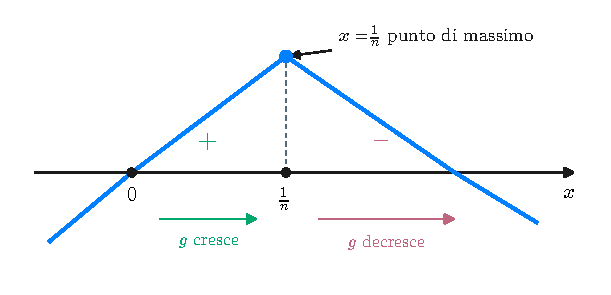
\includegraphics[width=0.82\textwidth]{immagini/segno_derivata}
\\[4pt]{\small\itshape Segno di $g'$ e andamento qualitativo di $g$ su $[0,+\infty[$.}
\end{center}

Quindi $g$ cresce su $[0, 1/n]$ e decresce su $[1/n, +\infty[$, e $x = 1/n$ è
punto di massimo assoluto (inoltre $g(0) = 0$ e $g(x) \to 0$ per
$x \to +\infty$). L'estremo superiore è un massimo e vale
\[
  M_n = g\!\left(\frac{1}{n}\right)
      = \frac{\dfrac{1}{n}}{1 + n^2 \cdot \dfrac{1}{n^2}}
      = \frac{1}{2n} \longrightarrow 0 .
\]

\paragraph{Conclusione.}
\[
  f_n \rightrightarrows 0 \quad \text{in } \mathbb{R} .
\]

% ---------------------------------------------------------------------
\needspace{12\baselineskip}
\subsection{Riepilogo}

\BoxBlue{Riepilogo del capitolo}{}{%
  \begin{itemize}
    \item Una successione di funzioni associa a ogni $n$ una funzione
          $f_n : I \to \mathbb{R}$; fissando $x$ si ottiene una successione numerica.
    \item \textbf{Convergenza puntuale}: $f_n(x) \to f(x)$ per ogni $x \in I$;
          l'indice $\nu$ dipende da $\varepsilon$ e da $x$.
    \item La convergenza puntuale \textbf{non} conserva la continuità
          ($x^n$ e $x^{1/n}$ su $[0,1]$).
    \item \textbf{Convergenza uniforme}: l'indice $\nu$ dipende solo da
          $\varepsilon$; graficamente, le $f_n$ entrano tutte nel tubo attorno a $f$.
    \item Criterio pratico:
          \[
            f_n \rightrightarrows f \text{ in } I
            \iff
            M_n = \sup_{x \in I} |f_n(x) - f(x)| \longrightarrow 0 .
          \]
    \item Uniforme $\Rightarrow$ puntuale, ma non viceversa: il limite uniforme,
          se esiste, è il limite puntuale.
    \item La convergenza uniforme dipende dall'insieme: spesso si ottiene
          restringendosi a insiemi limitati o allontanandosi dai punti di
          discontinuità del limite.
  \end{itemize}
}


% ---------------- Lezione 2 ----------------
% =====================================================================
%  Teorema di continuità del limite -- lezione 2
% =====================================================================

% [0:02:47]
\section{Teorema di continuità del limite}

\paragraph{In aula.} Fra le dimostrazioni viste oggi, quella del passaggio al limite
sotto il segno di integrale è indicata come possibile domanda d'esame; si dà per
noto tutto il materiale di Analisi I che vi compare (teorema di Weierstrass,
proprietà di confronto degli integrali, teorema dei carabinieri).

% [0:03:55]
\subsection{Enunciato}

La convergenza puntuale non conserva le proprietà delle funzioni che compongono la
successione: è proprio per questo che è stata introdotta la convergenza uniforme. Il
primo teorema che vediamo dice che, con la convergenza uniforme, la continuità si
trasmette al limite.

\Teorema{continuità del limite uniforme}{%
Siano
\begin{enumerate}
  \item $f_n\colon I\subseteq\mathbb{R}\to\mathbb{R}$ continua in $I$ per ogni $n$;
  \item $f_n\rightrightarrows f$ in $I$, con $f\colon I\subseteq\mathbb{R}\to\mathbb{R}$.
\end{enumerate}
Allora $f$ è continua in $I$.
}

% [0:05:50]
\BoxBlue{Osservazione}{}{%
Equivalentemente, la tesi si scrive come uno scambio di
limiti: per ogni $x_0\in I$
\begin{equation}
\lim_{x\to x_0} f(x)
= \lim_{x\to x_0}\Big(\lim_{n\to\infty} f_n(x)\Big)
= \lim_{n\to\infty}\Big(\lim_{x\to x_0} f_n(x)\Big)
= \lim_{n\to\infty} f_n(x_0)
= f(x_0).
\end{equation}
Nella prima uguaglianza si è usato che $f$ è il limite puntuale delle $f_n$, nella
terza che ciascuna $f_n$ è continua in $x_0$.
}

% [0:08:06]
\paragraph{In aula.} Il senso della formula precedente è questo: $f_n(x)$ dipende da
due variabili, l'indice $n$ e il punto $x$. In generale due operazioni di limite su
variabili diverse non si possono scambiare; \textbf{[In aula]} quando la convergenza
è uniforme, invece, i due limiti si possono invertire liberamente.

% [0:09:33]
\BoxBlue{Osservazione}{}{%
Il teorema \emph{non} è un ``se e solo se''. Se lo fosse,
lo studio della convergenza uniforme si ridurrebbe allo studio della continuità del
limite puntuale. Il controesempio è già noto: $f_n(x)=x/n$ converge puntualmente a
$f\equiv 0$, che è continua, ma la convergenza non è uniforme su tutto $\mathbb{R}$.
Quindi la continuità del limite puntuale non caratterizza la convergenza uniforme.
}

% [0:09:33]
\paragraph{In aula.} Il teorema si usa quasi sempre ``al negativo''. Se le $f_n$ sono
continue e il limite puntuale $f$ risulta discontinuo, allora si conclude
immediatamente che la convergenza \emph{non} è uniforme, senza calcolare alcun
$\sup$. È il caso di $f_n(x)=x^n$ su $[0,1]$ (figura~\ref{fig:01}), il cui limite
puntuale è
\[
f(x)=
\begin{cases}
0, & x\in[0,1[,\\[2pt]
1, & x=1.
\end{cases}
\]

\begin{figure}[htbp]\centering
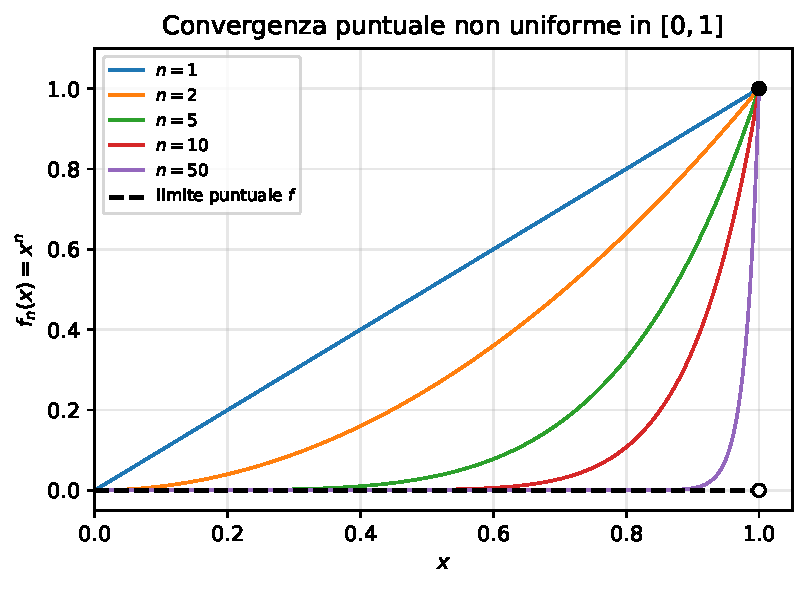
\includegraphics[width=0.6\linewidth]{figure/fig_01}
\caption{Andamento qualitativo di $f_n(x)=x^n$ su $[0,1]$ per alcuni valori di $n$ e
suo limite puntuale, discontinuo in $x=1$: essendo le $f_n$ continue, la convergenza
non può essere uniforme su $[0,1]$.}
\label{fig:01}
\end{figure}

% [0:10:34]
\paragraph{In aula.} Il teorema dice anche \emph{dove} conviene restringersi. Non
basta prendere un intervallo più piccolo a caso: su $[1/2,1]$ la discontinuità viene
di nuovo catturata e la convergenza resta non uniforme. Bisogna restringersi a un
insieme su cui il limite puntuale è continuo, per esempio $[0,a]$ con $a<1$. Questo è
il criterio pratico per cercare l'insieme più grande su cui si ha convergenza
uniforme.

% [0:11:43]
\subsection{Dimostrazione}

Sia $x_0\in I$; dimostriamo che $f$ è continua in $x_0$. Poiché $x_0$ è arbitrario,
seguirà la continuità su tutto $I$.

Dalle ipotesi:
\begin{itemize}
  \item dall'ipotesi 1, $f_n$ è continua in $x_0$, cioè
  \[
  \forall \epsilon>0 \;\; \exists\, \delta_n>0:\quad
  |f_n(x)-f_n(x_0)|<\epsilon \quad \forall x\in I,\ |x-x_0|<\delta_n;
  \]
  \item dall'ipotesi 2, $f_n\rightrightarrows f$ in $I$, cioè
  \[
  \forall \epsilon>0 \;\; \exists\, \nu_\epsilon>0:\quad
  |f_n(x)-f(x)|<\epsilon \quad \forall n>\nu_\epsilon,\ \forall x\in I.
  \]
\end{itemize}

\paragraph{In aula.} Nella prima definizione il $\delta$ dipende anche da $n$: ogni
$f_n$ ha il suo. Nella seconda, invece, l'indice $\nu_\epsilon$ è unico e va bene per
\emph{tutte} le $x$ contemporaneamente: è esattamente questo il contenuto in più
della convergenza uniforme, ed è l'unico ``ingrediente'' che serve ricordare della
dimostrazione.

Dobbiamo produrre il $\delta$ della continuità di $f$. Fissato $\epsilon>0$ partiamo
dalla quantità da stimare e inseriamo un termine $f_{\bar m}$ con
$\bar m>\nu_\epsilon$:
\begin{align*}
|f(x)-f(x_0)|
&= \big| f(x)-f_{\bar m}(x)+f_{\bar m}(x)-f_{\bar m}(x_0)+f_{\bar m}(x_0)-f(x_0)\big|\\
&\le \underbrace{|f(x)-f_{\bar m}(x)|}_{<\,\epsilon \ \text{per la 2}}
+\underbrace{|f_{\bar m}(x)-f_{\bar m}(x_0)|}_{<\,\epsilon \ \text{per la 1}}
+\underbrace{|f_{\bar m}(x_0)-f(x_0)|}_{<\,\epsilon \ \text{per la 2}}
\;<\;3\epsilon .
\end{align*}
Il primo e il terzo addendo si stimano con la convergenza uniforme (lo stesso indice
$\bar m$ va bene sia in $x$ sia in $x_0$); il secondo si stima con la continuità di
$f_{\bar m}$, che fornisce il $\delta_{\bar m}>0$ cercato. Poiché $\epsilon>0$ è
arbitrario, $f$ è continua in $x_0$. $\blacksquare$

\BoxBlue{Osservazione}{}{%
Se si preferisce ottenere esattamente $\epsilon$ al posto di
$3\epsilon$, basta applicare le tre stime con $\epsilon/3$.
}

\subsection{Un esempio con limite discontinuo in un punto}

\paragraph{Esempio.} Sia
\[
f_n(x)=\frac{\arctan\!\big(n(1+x^2)\big)}{1+n^2x^2}+x,
\qquad x\in[0,+\infty[.
\]
Il limite puntuale è
\[
\lim_{n\to\infty} f_n(x)=f(x)=
\begin{cases}
x, & x\in\,]0,+\infty[,\\[4pt]
\dfrac{\pi}{2}, & x=0,
\end{cases}
\]
perché per $x>0$ il numeratore resta limitato mentre il denominatore diverge, mentre
in $x=0$ resta $\arctan(n)\to\pi/2$. Il limite è discontinuo in $x=0$ e le $n$ sono
continue: per il teorema di continuità del limite non c'è convergenza uniforme su
$[0,+\infty[$ (figura~\ref{fig:08}).

Ci si restringe allora a $[a,+\infty[$ con $a>0$, dove il limite $f(x)=x$ è continuo.
Qui
\[
M_n=\sup_{x\in[a,+\infty[}\left|\frac{\arctan\!\big(n(1+x^2)\big)}{1+n^2x^2}\right|
\le \frac{\pi}{2}\,\sup_{x\in[a,+\infty[}\frac{1}{1+n^2x^2}
= \frac{\pi}{2}\cdot\frac{1}{1+n^2a^2}\longrightarrow 0,
\]
quindi $M_n\to 0$ per il teorema dei carabinieri e la convergenza è uniforme su
$[a,+\infty[$.

\BoxBlue{Osservazione}{}{%
La maggiorazione funziona perché l'arcotangente è
\emph{limitata}: si sostituisce il fattore scomodo con la sua limitazione $\pi/2$ e si
evita del tutto il calcolo esatto del $\sup$ (cioè lo studio della derivata).
}

\begin{figure}[htbp]\centering
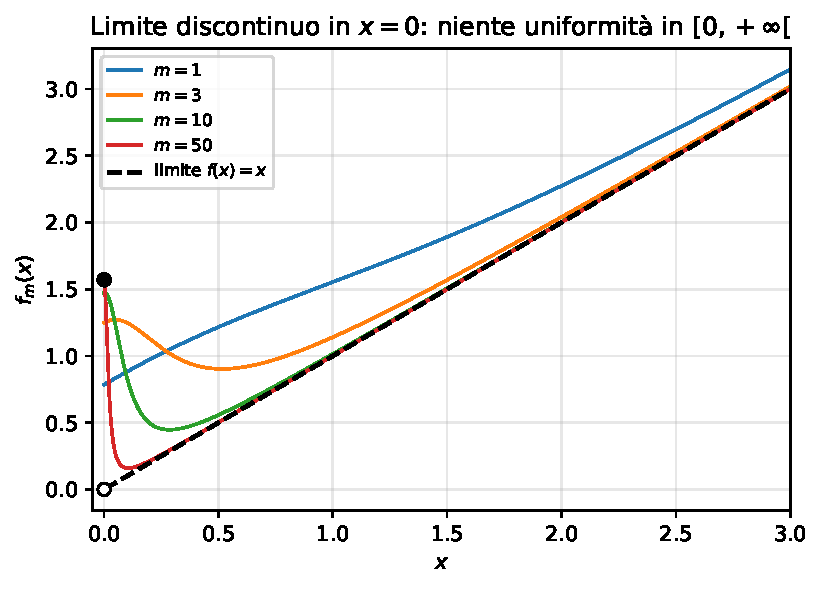
\includegraphics[width=0.6\linewidth]{figure/fig_08}
\caption{Andamento qualitativo di $f_n(x)=\arctan(n(1+x^2))/(1+n^2x^2)+x$ su
$[0,3]$: il limite puntuale vale $x$ per $x>0$ e $\pi/2$ in $x=0$.}
\label{fig:08}
\end{figure}

% [0:52:38]
\paragraph{In aula.} Un esercizio analogo, con lo stesso schema logico, è
$f_n(x)=\arctan(nx)$ su $\mathbb{R}$ (figura~\ref{fig:02}). Il limite puntuale è
\[
f(x)=
\begin{cases}
\pi/2, & x>0,\\
0, & x=0,\\
-\pi/2, & x<0,
\end{cases}
\]
discontinuo in $0$: niente convergenza uniforme su $\mathbb{R}$. Ci si può restringere
a $[a,+\infty[$ con $a>0$ \emph{oppure} a $]-\infty,-a]$ con $a>0$, ma non all'unione
dei due, perché l'insieme sarebbe sconnesso e si tornerebbe ad avere un limite
discontinuo [?]. Sul primo intervallo
\[
\sup_{x\ge a}\left|\arctan(nx)-\frac{\pi}{2}\right|
=\sup_{x\ge a}\left(\frac{\pi}{2}-\arctan(nx)\right)
=\frac{\pi}{2}-\arctan(na)\longrightarrow 0 .
\]
\textbf{[In aula]} Il valore assoluto si toglie scambiando i due termini (la
differenza ha segno costante) e il $\sup$ si trova \emph{senza} derivate: l'arcotangente
è crescente, quindi $\pi/2-\arctan(nx)$ è decrescente e il massimo si raggiunge
nell'estremo inferiore $x=a$. Il fatto che sia $a\neq 0$ è esattamente ciò che rende
il limite nullo.

\begin{figure}[htbp]\centering
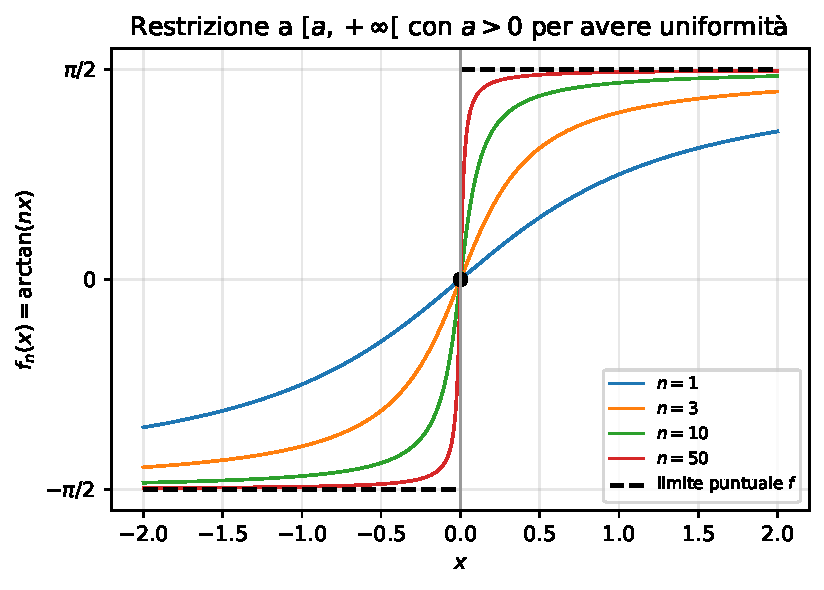
\includegraphics[width=0.6\linewidth]{figure/fig_02}
\caption{Andamento qualitativo di $f_n(x)=\arctan(nx)$: la convergenza è uniforme su
ogni $[a,+\infty[$ con $a>0$, ma non su $\mathbb{R}$.}
\label{fig:02}
\end{figure}

% =====================================================================
%  Passaggio al limite sotto il segno di integrale -- lezione 2
% =====================================================================

% [0:56:36]
\section{Passaggio al limite sotto il segno di integrale}

\subsection{Il problema}

Data una successione $f_n\colon[a,b]\to\mathbb{R}$ con limite $f$, ci si chiede se
\[
\int_a^b \Big(\lim_{n\to\infty} f_n(x)\Big)\,dx
\;=\;
\lim_{n\to\infty}\int_a^b f_n(x)\,dx .
\]
L'interesse pratico è evidente: a sinistra si integra la funzione limite, che di
solito è molto più semplice; a destra si integra ciascuna $f_n$ e poi si passa al
limite. Poterle scambiare significa poter approssimare un integrale difficile con una
successione di integrali facili.

\subsection{Enunciato}

\Teorema{passaggio al limite sotto il segno di integrale}{%
Siano
\begin{enumerate}
  \item $f_n\colon[a,b]\to\mathbb{R}$ continua per ogni $n$;
  \item $f_n\rightrightarrows f$ in $[a,b]$.
\end{enumerate}
Allora
\begin{equation}
\lim_{n\to\infty}\int_a^b f_n(x)\,dx
=\int_a^b \lim_{n\to\infty} f_n(x)\,dx
=\int_a^b f(x)\,dx .
\end{equation}
}

\BoxBlue{Osservazione}{}{%
Il limite $f$ che compare a destra è il limite puntuale
della successione; per il teorema di continuità del limite $f$ è continua, quindi
tutti gli integrali scritti hanno senso. Si noti anche che, mentre a sinistra si ha
una successione \emph{numerica} $I_n=\int_a^b f_n$, l'ipotesi di convergenza richiesta
sulle funzioni è quella uniforme: l'integrale definito è un numero, ma per controllarlo
serve un'informazione valida su tutto $[a,b]$ contemporaneamente.
}

\BoxBlue{Osservazione}{}{%
L'implicazione non si inverte: la validità del passaggio al
limite non garantisce la convergenza uniforme. Gli esempi che seguono chiariscono i
due lati della questione.
}

% [1:00:28]
\subsection{Due esempi}

\paragraph{Esempio 1.} $f_n(x)=n\,x\,(1-x^2)^n$, $x\in[0,1]$.

Limite puntuale: per $x=1$ si ha $f_n(1)=0$ per ogni $n$; per $0\le x<1$ la base
$1-x^2$ è minore di $1$, e l'esponenziale vince sulla potenza, quindi $f_n(x)\to 0$.
Dunque $f\equiv 0$ e
\[
\int_0^1 f(x)\,dx=0 .
\]
D'altra parte, riconoscendo a meno del fattore $-\tfrac{1}{2}$ la derivata di
$1-x^2$,
\[
\int_0^1 n\,x\,(1-x^2)^n\,dx
=-\frac{n}{2}\,\frac{(1-x^2)^{n+1}}{n+1}\bigg|_0^1
=0+\frac{n}{2(n+1)}
\;\xrightarrow[n\to\infty]{}\;\frac{1}{2}\neq 0 .
\]
Il passaggio al limite non vale, quindi per il teorema la convergenza \emph{non} può
essere uniforme (figura~\ref{fig:03}).

\begin{figure}[htbp]\centering
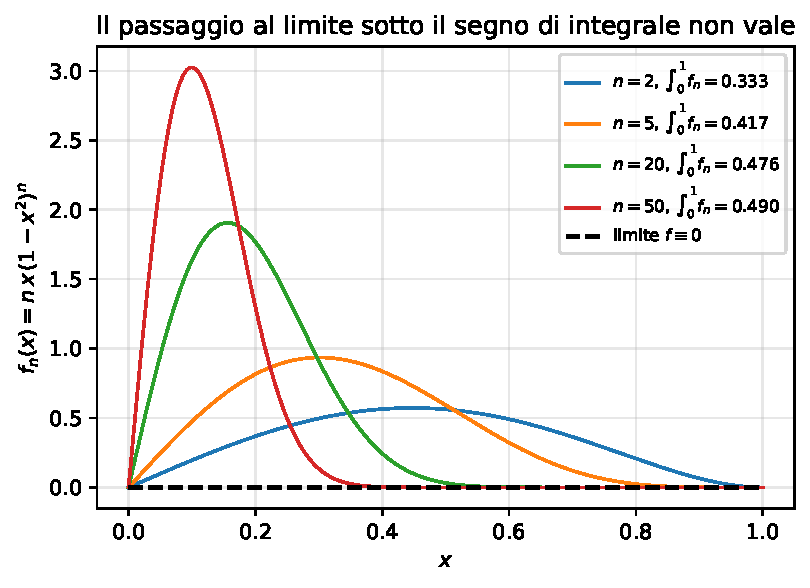
\includegraphics[width=0.6\linewidth]{figure/fig_03}
\caption{Andamento qualitativo di $f_n(x)=n\,x\,(1-x^2)^n$ su $[0,1]$: le funzioni
tendono puntualmente a zero, ma l'area sottesa tende a $1/2$.}
\label{fig:03}
\end{figure}

\paragraph{In aula.} Questo è il modo più economico di procedere: verificato che il
passaggio al limite fallisce, si conclude subito che la convergenza non è uniforme e
si evita completamente lo studio del $\sup$. (Per esercizio si può fare anche
direttamente: la derivata porta a una successione di massimi che non tende a zero.)

% [0:58:06]
\paragraph{Esempio 2.} $f_n(x)=n\,x\,e^{-nx}$, $x\in[0,1]$ (esercizio per casa, si
trova sul libro). Qui la convergenza è soltanto puntuale a $f\equiv 0$ — il massimo
vale $1/e$ per ogni $n$, raggiunto in $x=1/n$ — eppure il passaggio al limite vale,
perché $\int_0^1 f_n\to 0$ (figura~\ref{fig:04}).

\begin{figure}[htbp]\centering
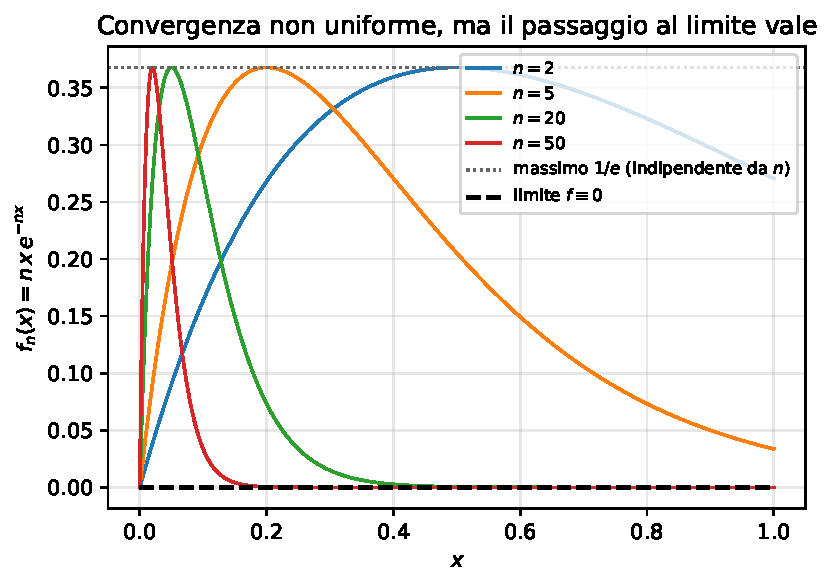
\includegraphics[width=0.6\linewidth]{figure/fig_04}
\caption{Andamento qualitativo di $f_n(x)=n\,x\,e^{-nx}$ su $[0,1]$: convergenza
puntuale non uniforme, ma gli integrali tendono comunque a zero.}
\label{fig:04}
\end{figure}

\BoxBlue{Osservazione}{}{%
I due esempi insieme dicono che: (i) la sola convergenza
puntuale, anche verso un limite ottimo (addirittura costante), non basta a garantire
il passaggio al limite; (ii) viceversa, il passaggio al limite può valere senza
convergenza uniforme, quindi l'implicazione del teorema non si inverte.
}

% [1:00:28]
\paragraph{In aula.} Le successioni $x^n$ e $x^{1/n}$ su $[0,1]$ non si prestano a
questo confronto: il loro limite è discontinuo in un estremo, e per evitarlo
bisognerebbe restringersi a $[0,a]$ con $a<1$, dove però la convergenza torna a essere
uniforme e non c'è più niente da osservare. L'esempio 1 è appunto una modifica di
$x^n$ costruita per aggirare questa difficoltà.

% [1:05:58]
\subsection{Dimostrazione}

Posto $I_n=\int_a^b f_n(x)\,dx$ e $I=\int_a^b f(x)\,dx$, si vuole mostrare che
$I_n\to I$: basta stimare $|I_n-I|$ con una quantità che tende a zero e concludere con
il teorema dei carabinieri. Si ha
\begin{align*}
|I_n-I|
&=\left|\int_a^b \big(f_n(x)-f(x)\big)\,dx\right|
&&\text{(linearità dell'integrale)}\\
&\le \int_a^b \big|f_n(x)-f(x)\big|\,dx
&&\text{(modulo dentro l'integrale)}\\
&\le \max_{x\in[a,b]}\big|f_n(x)-f(x)\big|\cdot(b-a)
&&\text{(confronto fra integrali)} .
\end{align*}
Il massimo esiste per il teorema di Weierstrass: la funzione $|f_n-f|$ è continua,
perché $f_n$ è continua per ipotesi e $f$ lo è per il teorema di continuità del limite.
Infine, per la convergenza uniforme, $\max_{[a,b]}|f_n-f|\to 0$, mentre $(b-a)$ è un
numero fissato: il prodotto tende a zero e, essendo $0\le|I_n-I|$, si conclude
$|I_n-I|\to 0$. $\blacksquare$

\paragraph{In aula.} Il passaggio con il massimo è quello che a scuola si chiama
``primo teorema della media'': in realtà è soltanto la proprietà di confronto fra
integrali, dato che la funzione è positiva e limitata superiormente dal suo massimo.
Al posto del massimo si può scrivere il $\sup$, che qui coincide.

% [1:10:49]
\paragraph{In aula.} La richiesta di convergenza uniforme è molto forte: moltissime
successioni convergono soltanto puntualmente e restano quindi fuori dal teorema. È
proprio questo il motivo per cui nel corso di Metodi verrà costruito un altro tipo di
integrale, con il quale il passaggio al limite si ottiene sotto ipotesi molto più
deboli.

% =====================================================================
%  Passaggio al limite sotto il segno di derivata -- lezione 2
% =====================================================================

% [1:12:12]
\section{Passaggio al limite sotto il segno di derivata}

\subsection{Perché il problema è più delicato}

La domanda analoga per le derivate è: vale
\[
\frac{d}{dx}\Big(\lim_{n\to\infty} f_n(x)\Big)
=\lim_{n\to\infty}\frac{d}{dx}f_n(x)\,?
\]

\paragraph{In aula.} Qui la situazione è molto più complessa che per l'integrale. Nel
caso dell'integrale gli oggetti $I_n$ erano \emph{numeri}: la convergenza era quella
di una successione numerica e non c'era ambiguità. Le derivate $f_n'$ sono invece
\emph{funzioni}, e una successione di funzioni può convergere in modi diversi, o non
convergere affatto. Può succedere che la funzione limite non sia derivabile anche se
tutte le $f_n$ lo sono; che le derivate non ammettano limite; che i due membri
esistano ma siano diversi. Servono quindi più ipotesi. I tre esempi che seguono
servono a capire quali.

% [1:16:37]
\subsection{Esempio 1: il limite può non essere derivabile}

\[
f_n(x)=\sqrt{x^2+\frac{1}{n}},\qquad x\in\mathbb{R}.
\]
Ogni $f_n$ è derivabile infinite volte su $\mathbb{R}$: il radicando è strettamente
positivo grazie al termine $1/n$, quindi il problema della radice in zero non si
presenta. Il limite puntuale è
\[
\lim_{n\to\infty} f_n(x)=|x|=f(x),
\]
che non è derivabile in $x=0$ (figura~\ref{fig:05}).

La convergenza è addirittura uniforme. Infatti, razionalizzando,
\[
\big|f_n(x)-|x|\big|
=\sqrt{x^2+\tfrac1n}-|x|
=\frac{1/n}{\sqrt{x^2+\tfrac1n}+|x|},
\]
quantità decrescente in $|x|$: il $\sup$ si ottiene in $x=0$ e vale
$\dfrac{1/n}{\sqrt{1/n}}=\dfrac{1}{\sqrt n}\to 0$.

\BoxBlue{Osservazione}{}{%
Dunque la sola convergenza uniforme delle $f_n$ non basta:
occorre chiedere qualcosa sulle \emph{derivate}.
}

\begin{figure}[htbp]\centering
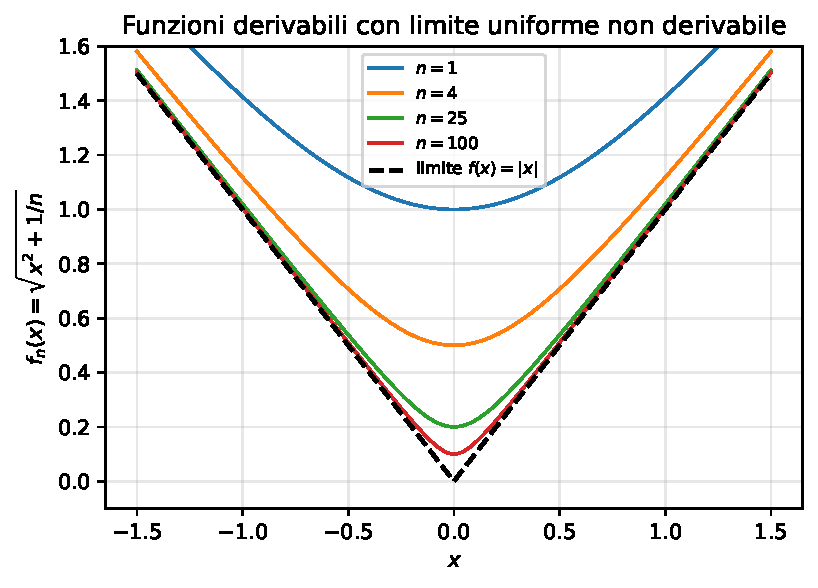
\includegraphics[width=0.6\linewidth]{figure/fig_05}
\caption{Andamento qualitativo di $f_n(x)=\sqrt{x^2+1/n}$: funzioni regolari che
convergono uniformemente a $|x|$, non derivabile in $x=0$.}
\label{fig:05}
\end{figure}

% [1:21:51]
\subsection{Esempio 2: le derivate possono non convergere}

\[
f_n(x)=\frac{\sin(nx)}{n},\qquad x\in\mathbb{R}.
\]
Si ha $f_n\rightrightarrows f\equiv 0$, e la verifica è immediata: $|\sin(nx)|\le 1$,
quindi $|f_n(x)|\le 1/n\to 0$ indipendentemente da $x$. Le $f_n$ sono derivabili
quante volte si vuole, quindi stavolta tutti i presupposti ci sono. Però
\[
f_n'(x)=\cos(nx),
\]
che per $x$ generico è oscillante e non ammette limite. Nei punti in cui il limite
esiste, per esempio $x=0$, si ha $f_n'(0)=1$ per ogni $n$, mentre $f'(0)=0$: i due
membri esistono ma sono diversi (figura~\ref{fig:06}).

\begin{figure}[htbp]\centering
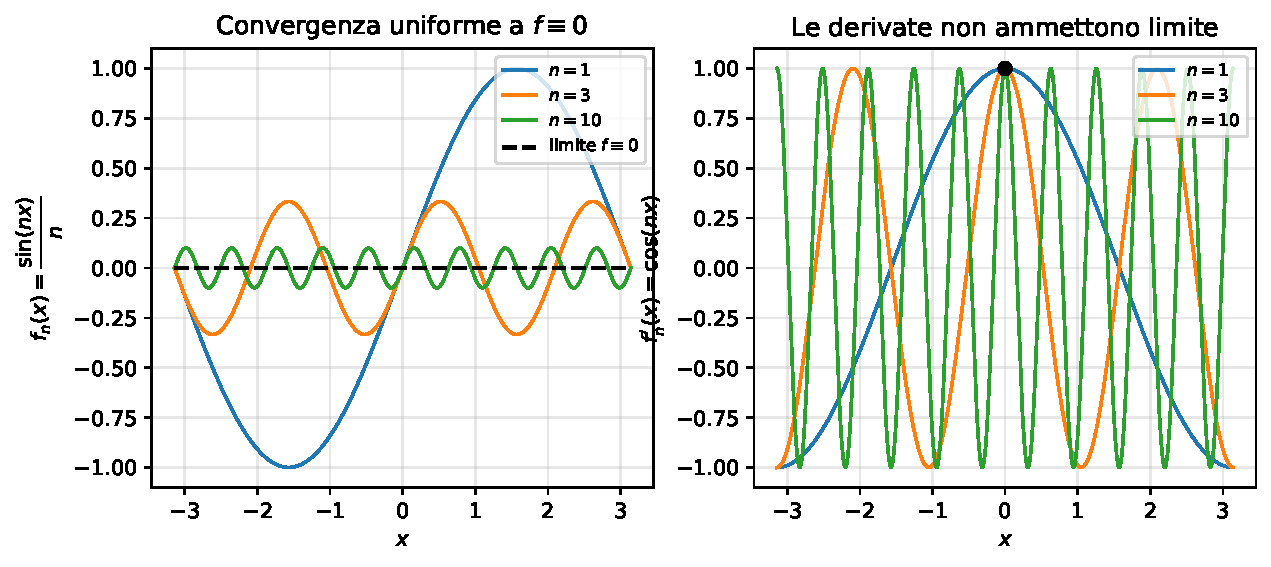
\includegraphics[width=0.85\linewidth]{figure/fig_06}
\caption{Andamento qualitativo di $f_n(x)=\sin(nx)/n$ (a sinistra) e della successione
delle derivate $f_n'(x)=\cos(nx)$ (a destra): convergenza uniforme delle $f_n$, nessun
limite per le derivate.}
\label{fig:06}
\end{figure}

% [1:25:48]
\subsection{Esempio 3: le derivate convergono, ma solo puntualmente}

\[
f_n(x)=\frac{x}{1+n^2x^2},\qquad x\in[0,1].
\]
Si ha $f_n\rightrightarrows f\equiv 0$ (per $x=0$ la funzione è nulla; per $x\neq 0$ il
denominatore diverge; la verifica dell'uniformità si fa come negli esempi precedenti),
quindi $f'\equiv 0$. Le derivate esistono per ogni $n$, perché il denominatore non si
annulla mai:
\[
f_n'(x)=\frac{1-n^2x^2}{(1+n^2x^2)^2}.
\]
Stavolta la successione delle derivate \emph{ammette} limite puntuale:
\[
f_n'(x)\longrightarrow
\begin{cases}
0, & x\neq 0,\\
1, & x=0,
\end{cases}
\]
e quindi
\[
\lim_{n\to\infty} f_n'(0)=1\neq 0=f'(0).
\]
Il passaggio al limite non vale. Il limite delle derivate è discontinuo in $0$ mentre
le $f_n'$ sono continue: per il teorema di continuità del limite la convergenza delle
derivate non è uniforme (figura~\ref{fig:07}).

\begin{figure}[htbp]\centering
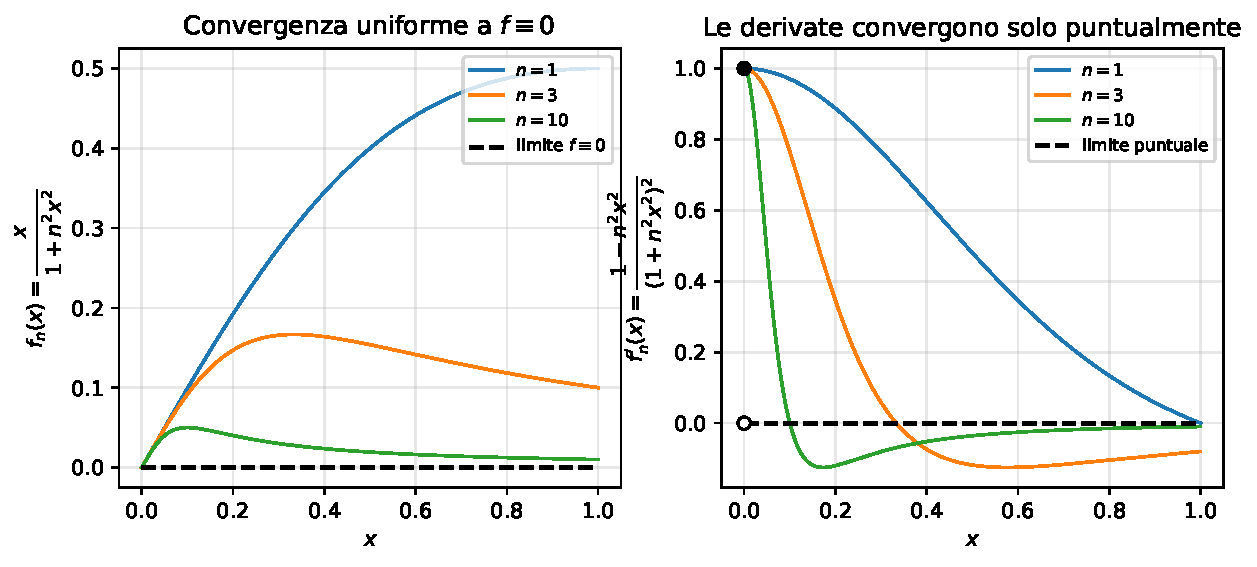
\includegraphics[width=0.85\linewidth]{figure/fig_07}
\caption{Andamento qualitativo di $f_n(x)=x/(1+n^2x^2)$ (a sinistra) e delle derivate
$f_n'(x)=(1-n^2x^2)/(1+n^2x^2)^2$ (a destra) su $[0,1]$: il limite delle derivate è
discontinuo in $x=0$.}
\label{fig:07}
\end{figure}

% [1:31:05]
\paragraph{In aula.} Il filo conduttore dei tre esempi è che in nessuno di essi si è
mai chiesto che la successione delle \emph{derivate} converga uniformemente: è questa
l'informazione che manca. Al contrario, nel terzo esempio si vede che quello che fanno
le $f_n$ è quasi irrilevante: sarà sufficiente saperne il comportamento in un solo
punto.

% [1:32:01]
\subsection{Enunciato}

\Teorema{passaggio al limite sotto il segno di derivata}{%
Siano
\begin{enumerate}
  \item $f_n\colon[a,b]\to\mathbb{R}$ con $f_n\in C^1([a,b])$ per ogni $n$;
  \item esista $x_0\in[a,b]$ tale che $\displaystyle\lim_{n\to\infty}f_n(x_0)=L\in\mathbb{R}$;
  \item esista $g\colon[a,b]\to\mathbb{R}$ tale che $f_n'\rightrightarrows g$ in $[a,b]$.
\end{enumerate}
Allora
\begin{enumerate}
  \item[T1)] $f_n\rightrightarrows f$ in $[a,b]$, per una opportuna $f\colon[a,b]\to\mathbb{R}$;
  \item[T2)] $f\in C^1([a,b])$ e $f'=g$, cioè
\end{enumerate}
\begin{equation}
\frac{d}{dx}\Big(\lim_{n\to\infty} f_n(x)\Big)
=\lim_{n\to\infty}\frac{d}{dx}f_n(x).
\end{equation}
}

\BoxBlue{Osservazione}{}{%
$C^1([a,b])$ significa: derivabile con derivata continua.
L'ipotesi $C^1$ si può indebolire chiedendo solo la derivabilità, ma l'enunciato e
soprattutto la dimostrazione diventano sensibilmente più complicati; nei testi si
trova anche quella versione.
}

\BoxBlue{Osservazione}{}{%
L'ipotesi 2 è sorprendentemente debole: delle $f_n$ non si
chiede nulla, se non che convergano \emph{in un solo punto}. L'ipotesi sostanziale è
la 3, la convergenza uniforme delle derivate. Si noti che la convergenza (anche
uniforme) delle $f_n$, che negli esempi c'era sempre, non è servita a nulla.
}

\subsection{Dimostrazione}
% [0:01:19]
Questo è il più complesso dei tre teoremi di passaggio al limite, perché li \emph{usa}
entrambi: il teorema di continuità del limite serve a dire che $g$ è continua, quello di
passaggio al limite sotto il segno di integrale a costruire $f$. Chi non conosce i primi
due non può dimostrare questo.

\paragraph{Passo 1: costruire $f$.} La funzione $f$ non è data, va costruita: le ipotesi
danno un'informazione sulla successione in un solo punto, $x_0$. Poiché $f_n\in C^1$
— ipotesi che qui viene sfruttata in modo essenziale — la sua derivata $f_n'$ è continua
e quindi integrabile: per il teorema fondamentale del calcolo integrale
\begin{equation}
f_n(x)=f_n(x_0)+\int_{x_0}^{x} f_n'(t)\,dt,\qquad x\in[a,b].
\end{equation}
% [0:02:50]
La riscrittura sembra artificiosa — si parte da una funzione che c'è già e la si riscrive
in una forma più complicata — ma è proprio ciò che conviene, perché fa \emph{comparire una
funzione}: il membro di destra ammette limite.
\begin{itemize}
  \item $f_n(x_0)\to L$ per l'ipotesi 2;
  \item $\displaystyle\int_{x_0}^{x} f_n'(t)\,dt\to\int_{x_0}^{x} g(t)\,dt$ per il
  teorema di passaggio al limite sotto il segno di integrale, applicabile grazie alle
  ipotesi 1 e 3 (le $f_n'$ sono continue e convergono uniformemente a $g$).
\end{itemize}
Dunque $f_n$ converge puntualmente alla funzione
\begin{equation}
f(x)=L+\int_{x_0}^{x} g(t)\,dt .
\end{equation}

% [1:41:50]
\paragraph{Passo 2: la tesi T2.} La $g$ è continua, perché è limite uniforme delle
funzioni continue $f_n'$ (teorema di continuità del limite). Allora
$x\mapsto\int_{x_0}^{x} g(t)\,dt$ è la funzione integrale di una funzione continua,
quindi per il teorema fondamentale del calcolo è derivabile con derivata $g(x)$; il
termine $L$ è una costante e ha derivata nulla. Perciò
\[
f'(x)=g(x)\quad\text{in }[a,b],
\]
e poiché $g$ è continua si ha $f\in C^1([a,b])$. Questa è esattamente la tesi T2.
% [0:09:40]
Conviene fissare la distinzione che si è appena usata: se l'integranda è \emph{solo
integrabile}, della funzione integrale si può concludere soltanto la continuità; se
l'integranda è \emph{continua}, si guadagna di più, cioè la derivabilità con derivata
l'integranda — ed è precisamente ciò che serve qui.

% [1:45:23]
\paragraph{Passo 3: la tesi T1.} Resta da mostrare che la convergenza $f_n\to f$ è
uniforme. L'idea è maggiorare $|f_n(x)-f(x)|$ con una quantità che non dipende da $x$ e
che tende a zero in $n$. Sottraendo le due rappresentazioni integrali e usando la
disuguaglianza triangolare:
\begin{align*}
0\le |f_n(x)-f(x)|
&\le |f_n(x_0)-L|+\left|\int_{x_0}^{x}\big(f_n'(t)-g(t)\big)\,dt\right|\\
&\le |f_n(x_0)-L|+\int_a^b \big|f_n'(t)-g(t)\big|\,dt\\
&\le |f_n(x_0)-L|+\max_{t\in[a,b]}\big|f_n'(t)-g(t)\big|\cdot(b-a).
\end{align*}
% [0:06:54]
Nel passaggio alla seconda riga il punto delicato è il \emph{doppio modulo}: il valore
assoluto si può portare \emph{dentro} l'integrale (maggiorando), ma quello \emph{fuori} va
lasciato. Il motivo è che gli estremi $x_0$ e $x$ sono in ordine ignoto: se fosse $x<x_0$
l'integrale cambierebbe segno e si starebbe maggiorando una quantità positiva con una
negativa, il che non è lecito. Quando gli estremi sono variabili, dunque, si può mettere
il modulo dentro ma non si può togliere quello fuori.
% [0:08:19]
Solo a questo punto, essendo l'integranda positiva, ci si libera della dipendenza da $x$
\emph{allargando} l'intervallo di integrazione a tutto $[a,b]$.

Il membro di destra \emph{non dipende da $x$}: il primo addendo tende a zero per
l'ipotesi 2, il secondo per l'ipotesi 3. Passando al $\sup$ su $x\in[a,b]$ la
maggiorazione si conserva, quindi
\[
0\le\sup_{x\in[a,b]}|f_n(x)-f(x)|\longrightarrow 0,
\]
cioè $f_n\rightrightarrows f$. $\blacksquare$

Il punto cruciale è proprio che la maggiorazione sia \emph{indipendente da $x$}: solo così
sopravvive al passaggio al $\sup$ e permette di concludere con il teorema dei carabinieri,
senza calcolare alcuna derivata. Se la quantità maggiorante dipendesse da $x$, l'argomento
non funzionerebbe.



% =====================================================================
%  Analisi Matematica II — Lezione 3 (seguito)
%  Inizio delle serie di funzioni (la prima parte della lezione è in
%  discontinuita-e-criteri-di-cauchy.tex).
%  Frammento da includere con \input; richiede amsmath, amssymb, graphicx.
% =====================================================================

% [0:29:08]
\section{Serie di funzioni}

% [0:32:00]
\subsection{Definizione}

\paragraph{Definizione.} Sia $f_n:I\subseteq\mathbb{R}\to\mathbb{R}$ per ogni
$n\in\mathbb{N}$. Si chiama \emph{serie di funzioni} di termine generale $f_n(x)$, e si
scrive
\begin{equation}
\sum_{n=1}^{+\infty}f_n(x),
\end{equation}
la successione di funzioni delle \emph{somme parziali}
\begin{equation}
S_1(x)=f_1(x),\qquad S_2(x)=f_1(x)+f_2(x)=S_1(x)+f_2(x),\qquad\dots
\end{equation}
e, in generale,
\begin{equation}
S_n(x)=S_{n-1}(x)+f_n(x).
\end{equation}
Si dice che la serie \emph{converge puntualmente} alla somma $S(x)$ in $I$ se
$S_n\to S$ puntualmente in $I$; si dice che \emph{converge uniformemente} a $S(x)$ in $I$
se $S_n\rightrightarrows S$ in $I$.

\paragraph{Osservazione.} Come per le successioni, la convergenza uniforme implica quella
puntuale.

% [0:29:08]
\paragraph{In aula.} La teoria delle serie di funzioni è, nelle parole della docente,
``povera'': a differenza delle serie numeriche, dove si dispone di molti criteri, lo studio
di una serie di funzioni generica può essere un esercizio molto complesso. Il motivo è che
la convergenza uniforme richiede di conoscere $S$, e già in Analisi I le uniche serie di
cui si sapeva calcolare la somma erano le geometriche e le telescopiche. L'obiettivo vero
del corso non sono le serie generiche ma le \emph{serie di potenze}, cioè quelle che hanno
la forma del polinomio di Taylor: la definizione generale serve per arrivarci.

% [0:30:38]
\paragraph{In aula.} I tipi di convergenza saranno quattro: puntuale, uniforme, assoluta e
totale. Inoltre l'insieme $I$ è scritto come sottoinsieme di $\mathbb{R}$, ma fra poco si
lavorerà con sottoinsiemi di $\mathbb{R}^2$: la definizione si trasporta senza modifiche.

% [0:34:47]
\paragraph{In aula.} Rispetto ad Analisi I non si parla più di \emph{carattere} della
serie: qui si tratta soltanto di stabilire se c'è convergenza e di che tipo. Dire che la
serie converge puntualmente significa che, fissato $x$, la serie numerica corrispondente
converge.

% [0:36:15]
\subsection{Esempio 1: la serie geometrica}

\paragraph{Esempio.} Si studi la convergenza puntuale e uniforme di
\begin{equation}
\sum_{n=0}^{+\infty}x^n,\qquad x\in\mathbb{R}.
\end{equation}

\emph{Convergenza puntuale.} È la serie geometrica di ragione $x$: converge puntualmente
se e solo se $|x|<1$, con somma
\begin{equation}
S(x)=\frac{1}{1-x},\qquad x\in\,]-1,1[\,.
\end{equation}

\emph{Convergenza uniforme in $]-1,1[$.} Dalla formula della progressione geometrica,
$S_n(x)=\dfrac{1-x^{\,n+1}}{1-x}$, e quindi
\begin{equation}
\sup_{]-1,1[}\big|S_n(x)-S(x)\big|
=\sup_{]-1,1[}\left|\frac{1-x^{\,n+1}}{1-x}-\frac{1}{1-x}\right|
=\sup_{]-1,1[}\frac{|x|^{\,n+1}}{1-x}=+\infty ,
\end{equation}
perché per $x\to1^-$ il numeratore tende a $1$ e il denominatore a $0^+$. Dunque
\[
S_n\to S\ \text{puntualmente in }]-1,1[,\qquad S_n\not\rightrightarrows S\ \text{in }]-1,1[.
\]

\emph{Come recuperare l'uniformità.} Come per le successioni, ci si allontana dagli
estremi: per ogni $r$ con $0<r<1$ si ha
\begin{equation}
\sup_{[-r,r]}\big|S_n(x)-S(x)\big|\le\frac{r^{\,n+1}}{1-r}\longrightarrow 0,
\end{equation}
quindi la convergenza è uniforme su ogni compatto $\{|x|\le r\}\subset\,]-1,1[$.

% [0:40:04]
\paragraph{In aula.} La serie geometrica di Analisi I era già, senza dirlo, una serie di
funzioni: bastava chiamare $x$ la ragione $q$. È il primo esempio da tenere presente anche
perché $x^n$ è già il prototipo del termine di una serie di potenze.

% [0:43:56]
\paragraph{In aula.} Il motivo per cui il sup esplode è tutto nel denominatore: per quanto
$|x|^{\,n+1}$ diventi piccolo, avvicinandosi a $1$ il denominatore $1-x$ manda il rapporto
all'infinito. L'intervallo aperto è il problema; appena ci si mette in un compatto più
piccolo, tutto funziona.

% [0:50:30]
\subsection{Esempio 2: una serie a segni alterni}

\paragraph{Esempio.} Si studi la convergenza puntuale, uniforme e assoluta di
\begin{equation}
\sum_{n=1}^{+\infty}(-1)^n\,\frac{x^2+n}{n^2},\qquad x\in[-1,1].
\end{equation}

\emph{Convergenza puntuale.} Si applica il criterio di Leibniz, fissato $x$. Posto
\begin{equation}
a_n(x)=\frac{x^2+n}{n^2}=\frac{x^2}{n^2}+\frac{1}{n},
\end{equation}
si vede subito che $a_n(x)>0$, che $a_n(x)$ è decrescente in $n$ (entrambi gli addendi lo
sono, e la monotonia richiesta è in $n$, non in $x$) e che $a_n(x)\to0$. Quindi la serie
converge puntualmente per ogni $x\in[-1,1]$.

\emph{Convergenza uniforme.} Non conosciamo $S$, ma per le serie a segni alterni viene in
aiuto la \emph{stima del resto}: $|S_n(x)-S(x)|\le a_{n+1}(x)$. Allora
\begin{equation}
\sup_{[-1,1]}\big|S_n(x)-S(x)\big|\le\sup_{[-1,1]}a_{n+1}(x)
=\sup_{[-1,1]}\frac{x^2+n+1}{(n+1)^2}=\frac{n+2}{(n+1)^2}\longrightarrow0,
\end{equation}
dove il sup si calcola in $x=\pm1$ perché $x$ varia in un compatto. Dunque la serie
converge uniformemente in $[-1,1]$.

% [0:51:32]
\paragraph{In aula.} La stima del resto — che in Analisi I poteva sembrare un dettaglio —
è esattamente ciò che rende le serie a segni alterni comode anche in Analisi II: maggiora
$|S_n-S|$ senza richiedere di conoscere $S$, e riporta il problema allo studio di una
successione. Se il primo termine trascurato non tende a zero uniformemente, però, il
criterio non dice nulla e ci si ferma.

% [0:55:22]
\subsection{Convergenza assoluta}

\paragraph{Definizione.} Sia $f_n:I\subseteq\mathbb{R}\to\mathbb{R}$. La serie
$\sum_{n=1}^{+\infty}f_n$ \emph{converge assolutamente} in $I$ se converge puntualmente la
serie dei moduli
\begin{equation}
\sum_{n=1}^{+\infty}|f_n(x)| .
\end{equation}

\paragraph{Esempio.} La serie dell'Esempio 2 non converge assolutamente: per ogni
$x\in[-1,1]$
\begin{equation}
\sum_{n=1}^{+\infty}\frac{x^2+n}{n^2}\ \ge\ \sum_{n=1}^{+\infty}\frac{1}{n},
\end{equation}
che diverge. Si ha quindi convergenza uniforme \emph{senza} convergenza assoluta.

% [0:56:58]
\paragraph{In aula.} Questo esempio servirà ancora: mostra che fra convergenza assoluta e
convergenza uniforme non c'è alcun legame, in nessuno dei due versi. La serie dei moduli,
qui, si comporta in sostanza come la serie armonica generalizzata.

% [0:59:23]
\subsection{Criteri di Cauchy per le serie di funzioni}

Si ottengono scrivendo i criteri di Cauchy per la successione delle somme parziali,
osservando che
\[
S_{n+p}(x)-S_n(x)=f_{n+1}(x)+\dots+f_{n+p}(x)
\]
è il \emph{resto} della serie.

\paragraph{Criterio di Cauchy (convergenza puntuale).}
Sia $f_n:I\subseteq\mathbb{R}\to\mathbb{R}$ per ogni $n\in\mathbb{N}$:
$\sum_{n=1}^{+\infty}f_n(x)$
converge puntualmente in $I$ se e solo se
\begin{equation}
\forall x\in I,\ \forall\varepsilon>0\ \ \exists\,\nu_{x,\varepsilon}:\quad
\big|f_{n+1}(x)+\dots+f_{n+p}(x)\big|<\varepsilon
\qquad\forall p\in\mathbb{N},\ \forall n>\nu_{x,\varepsilon}.
\end{equation}

\paragraph{Criterio di Cauchy (convergenza uniforme).}
Sia $f_n:I\subseteq\mathbb{R}\to\mathbb{R}$ per ogni $n\in\mathbb{N}$:
$\sum_{n=1}^{+\infty}f_n(x)$
converge uniformemente in $I$ se e solo se
\begin{equation}
\forall\varepsilon>0\ \ \exists\,\nu_{\varepsilon}:\quad
\big|f_{n+1}(x)+\dots+f_{n+p}(x)\big|<\varepsilon
\qquad\forall p\in\mathbb{N},\ \forall n>\nu_{\varepsilon},\ \forall x\in I.
\end{equation}

% [1:01:27]
\paragraph{In aula.} Non c'è niente da dimostrare: sono i criteri di Cauchy per le
successioni, applicati alle somme parziali. Il primo è addirittura il criterio di Analisi I
scritto punto per punto. Si introducono adesso perché da essi escono immediatamente le
condizioni di convergenza.

% [1:02:56]
\subsection{Condizione necessaria per la convergenza uniforme}

\paragraph{Teorema.} Sia $f_n:I\subseteq\mathbb{R}\to\mathbb{R}$ per ogni $n$. Se
$\sum_{n=1}^{+\infty}f_n(x)$ converge uniformemente in $I$, allora
\begin{equation}
f_n\rightrightarrows 0\quad\text{in }I .
\end{equation}

\paragraph{Dimostrazione.} Si applica il criterio di Cauchy uniforme con $p=1$: resta
$|f_{n+1}(x)|<\varepsilon$ per ogni $n>\nu_\varepsilon$ e per ogni $x\in I$, che è
esattamente la definizione di $f_n\rightrightarrows0$. $\blacksquare$

% [1:02:56]
\paragraph{In aula.} È lo stesso meccanismo di Analisi I, dove si scriveva
$a_n=S_n-S_{n-1}$ per dedurre che il termine generale di una serie convergente tende a
zero; qui, non potendo usare quell'argomento nella versione uniforme, lo si ottiene
direttamente da Cauchy. La versione puntuale (il termine generale tende a zero
puntualmente) è ancora Analisi I, applicata $x$ per $x$.

% [1:08:07]
\subsection{Convergenza totale e criterio di Weierstrass}

\paragraph{Definizione (convergenza totale).} Sia
$f_n:I\subseteq\mathbb{R}\to\mathbb{R}$. La serie $\sum_{n=1}^{+\infty}f_n(x)$ converge
\emph{totalmente} in $I$ se esiste una successione numerica $M_n>0$ tale che
\begin{enumerate}
  \item $|f_n(x)|\le M_n$ per ogni $n\in\mathbb{N}$ e per ogni $x\in I$;
  \item la serie numerica $\sum_{n=1}^{+\infty}M_n$ converge.
\end{enumerate}

\paragraph{Osservazione.} Valgono le implicazioni
\begin{equation}
\text{TOTALE}\ \Longrightarrow\ \text{ASSOLUTA}\ \Longrightarrow\ \text{PUNTUALE},
\end{equation}
la prima perché $\sum|f_n(x)|$ è maggiorata da $\sum M_n$, la seconda per il criterio di
Analisi I.

% [1:08:07]
\paragraph{In aula.} L'idea della definizione è semplice: non potendo calcolare
$\sup_I|S_n-S|$, si maggiora la serie dei moduli con una serie numerica convergente, cioè
con qualcosa che \emph{non dipende da $x$}. Non basta la convergenza assoluta: serve una
maggiorazione uniforme rispetto a $x$.

% [1:12:16]
\paragraph{In aula.} Il numero $M_n$ non è altro che il $m_n=\sup_I|f_n(x)|$ che si usava
per la convergenza uniforme (con funzione limite nulla). Non è obbligatorio prendere
proprio il sup: va bene qualunque maggiorante più semplice da calcolare, come si fa negli
esercizi cercando una maggiorazione asintotica comoda.

% [1:14:55]
\paragraph{Teorema (criterio di Weierstrass).} Sia
$f_n:I\subseteq\mathbb{R}\to\mathbb{R}$ per ogni $n$. Se $\sum_{n=1}^{+\infty}f_n$
converge totalmente in $I$, allora converge uniformemente in $I$.

\paragraph{Dimostrazione.} Per ipotesi esiste $M_n>0$ con $|f_n(x)|\le M_n$ per ogni $n$ e
ogni $x\in I$, e $\sum M_n$ converge. Per il criterio di Cauchy applicato alla serie
\emph{numerica} $\sum M_n$,
\[
\forall\varepsilon>0\ \exists\,\nu:\quad M_{n+1}+\dots+M_{n+p}<\varepsilon
\qquad\forall p\in\mathbb{N},\ \forall n>\nu,
\]
e $\nu$ non dipende da $x$ perché i $M_n$ sono numeri. Allora, per la disuguaglianza
triangolare,
\begin{equation}
\big|f_{n+1}(x)+\dots+f_{n+p}(x)\big|\le|f_{n+1}(x)|+\dots+|f_{n+p}(x)|
\le M_{n+1}+\dots+M_{n+p}<\varepsilon
\end{equation}
per ogni $p\in\mathbb{N}$, ogni $n>\nu$ e \emph{ogni} $x\in I$. Vale dunque il criterio di
Cauchy per la convergenza uniforme, e la serie converge uniformemente in $I$.
$\blacksquare$

% [1:21:06]
\paragraph{In aula.} Il criterio di Cauchy viene usato due volte e nei due versi opposti:
in un verso per le serie numeriche (da $\sum M_n$ convergente si ricava la condizione di
Cauchy), nell'altro per le serie di funzioni (dalla condizione di Cauchy si ricava la
convergenza uniforme). È l'unico strumento che permette di dimostrare la convergenza
uniforme senza conoscere la somma.

% [1:16:17]
\paragraph{In aula.} Lo schema delle implicazioni si può leggere come due binari
(figura~\ref{fig:09}): dalla convergenza totale si arriva alla puntuale passando o per
l'assoluta o per l'uniforme, ma fra assoluta e uniforme non c'è alcun legame. Da qui una
conseguenza pratica usata negli esercizi: nell'Esempio 2 non c'è convergenza assoluta,
quindi non può esserci convergenza totale, ed è inutile mettersi a studiarla.

% [1:22:33]
\paragraph{In aula.} Schema operativo per studiare una serie di funzioni: non si cerca $S$
(quasi mai si trova). Si comincia dalla condizione necessaria, cioè si controlla se
$f_n\to0$ uniformemente; quel calcolo produce già $\sup_I|f_n|$, cioè il candidato $M_n$,
e a quel punto si studia direttamente la convergenza totale. Se la totale c'è, l'esercizio
è finito; se non c'è, si torna al punto di partenza.

\begin{figure}[htbp]
\centering
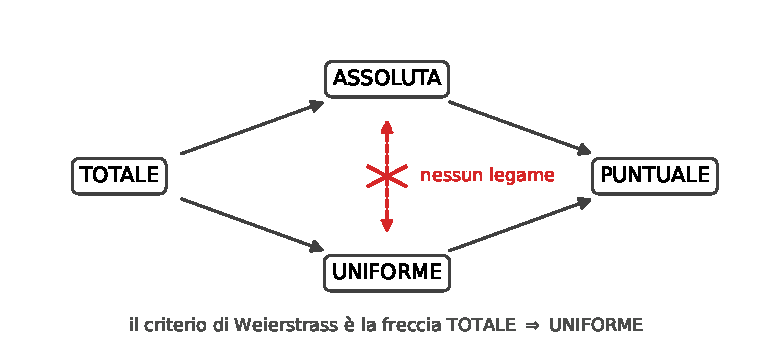
\includegraphics[width=0.7\linewidth]{figure/fig_09}
\caption{Relazioni fra i quattro tipi di convergenza per le serie di funzioni (schema
disegnato alla lavagna). Dalla convergenza totale si raggiunge la puntuale lungo due
``binari'' indipendenti; fra convergenza assoluta e convergenza uniforme non sussiste
alcuna implicazione.}
\label{fig:09}
\end{figure}

% [1:29:34]
\subsection{Teorema di integrazione per serie}

\paragraph{Teorema.} Sia $f_n:[a,b]\to\mathbb{R}$ continua per ogni $n\in\mathbb{N}$. Se
$\sum_{n=1}^{+\infty}f_n(x)$ converge uniformemente a $S(x)$ in $[a,b]$, allora
\begin{equation}
\sum_{n=1}^{+\infty}\int_a^b f_n(x)\,dx=\int_a^b\sum_{n=1}^{+\infty}f_n(x)\,dx
=\int_a^b S(x)\,dx .
\end{equation}

\paragraph{Dimostrazione.} Si considera la somma parziale $n$-esima della serie numerica a
primo membro:
\begin{align*}
I_n&=\int_a^b f_1(x)\,dx+\dots+\int_a^b f_n(x)\,dx\\
&=\int_a^b\big(f_1(x)+\dots+f_n(x)\big)\,dx=\int_a^b S_n(x)\,dx,
\end{align*}
dove si è usata la linearità dell'integrale. Per ipotesi $S_n\rightrightarrows S$ in
$[a,b]$ e ogni $S_n$ è continua (somma finita di funzioni continue), quindi si può passare
al limite sotto il segno di integrale:
\begin{equation}
\lim_{n\to+\infty}I_n=\lim_{n\to+\infty}\int_a^b S_n(x)\,dx
=\int_a^b\lim_{n\to+\infty}S_n(x)\,dx=\int_a^b S(x)\,dx . \qquad\blacksquare
\end{equation}

% [1:31:56]
\paragraph{In aula.} La dimostrazione è immediata una volta capiti i teoremi sulle
successioni: tutto consiste nel riconoscere che la somma parziale della serie degli
integrali è l'integrale della somma parziale. Si potrebbe premettere anche il teorema di
continuità del limite per dire che $S$ è continua — $S_n$ è somma di funzioni continue e
converge uniformemente — ma è così immediato che lo si usa direttamente.

% [1:35:44]
\paragraph{In aula (esercizio).} Allo stesso modo, dai teoremi sulle successioni di
funzioni si ricava il \emph{teorema di derivazione per serie}: la docente lo lascia da
scrivere come esercizio, dicendo che è ``la copia conforme'' dell'altro teorema, enunciato
sulle serie. Traccia: se $f_n\in C^1([a,b])$ per ogni $n$, se esiste $x_0\in[a,b]$ tale
che $\sum_n f_n(x_0)$ converge e se $\sum_n f_n'$ converge uniformemente in $[a,b]$,
allora $\sum_n f_n$ converge uniformemente a una somma $S\in C^1([a,b])$ e
\[
S'(x)=\sum_{n=1}^{+\infty}f_n'(x),\qquad x\in[a,b].
\]

% =====================================================================
% DUBBI:
%
% - Indici: su tutto il testo gli indici trascritti dall'OCR come "m" sono stati
%   normalizzati a "n" (indicazione esplicita). Fa eccezione il criterio di Cauchy,
%   dove servono due indici distinti n, m (audio [0:18:03]).
% - p.2 e p.3 degli appunti: il criterio di Cauchy è trascritto dall'OCR come
%   |f_n(x) - f(x)| < eps; è un errore di trascrizione, la quantità corretta è
%   |f_n(x) - f_m(x)| (audio [0:18:03] e [0:23:08]). Corretto nel testo.
% - p.1: "f è ricucibilmente continua" -> "f è sicuramente continua" (audio [0:02:50]).
% - p.1: "g'(eps) = g(eps)" -> derivata della funzione integrale di g uguale a g(x);
%   la variabile muta trascritta come epsilon è t.
% - p.4: l'OCR scrive sup |x|^{n+1}/(1-x) -> +infinito come se fosse un limite in n;
%   in realtà il sup su ]-1,1[ vale +infinito per ogni n fissato (audio [0:43:56]).
% - p.4: la riga "|x| < 1, per ogni M > 0, esiste eps > 0" è illeggibile; ricostruita
%   dall'audio [0:45:15] come restrizione ai compatti |x| <= r con 0 < r < 1.
% - p.5: "b.m.z." negli appunti è quasi certamente "Leibniz" (criterio per le serie a
%   segni alterni), confermato dall'audio [0:51:32].
% - p.5: la stima del resto è scritta come |S_n - S| < 1/(n+1); la forma generale usata
%   qui è |S_n - S| <= a_{n+1}, che nell'esempio dà (n+2)/(n+1)^2 (audio [0:53:57]).
% - p.6: nei criteri di Cauchy per le serie gli indici N e n sono mescolati; normalizzati
%   a n (resto f_{n+1} + ... + f_{n+p}, per ogni n > nu).
% - p.7: "esiste nu > 0" -> nu è un indice in N; "alpha_{n+1}" di p.8 è M_{n+1}.
% - p.8: "AB Bioma usato 2 volte il criterio di Cauchy" -> "Abbiamo usato 2 volte il
%   criterio di Cauchy".
% - Figure: le immagini figure/Analisi_II_p001_1.png, p001_2.png, p005_2.png,
%   p005_5.png sono loghi e segni decorativi degli appunti, non figure matematiche;
%   non ricostruite. L'unica figura ricostruita (fig_01) è lo schema dei "binari"
%   delle implicazioni fra i tipi di convergenza, effettivamente disegnato alla
%   lavagna [1:16:17].
% - Teorema di derivazione per serie: enunciato solo annunciato a lezione [1:35:44] e
%   lasciato per esercizio; la traccia riportata è la trasposizione alle serie del
%   teorema sulle successioni, da verificare con la dispensa della docente.
% - Note organizzative: la frase dell'audio [1:34:21] sulla prossima lezione ("lunedì")
%   è disturbata e non si capisce se sia una data di lezione o di ricevimento [?].
% - Audio [0:22:33]: accenno a uno strumento di registrazione/trascrizione usato in
%   aula; passaggio confuso, riportato solo nella sostanza [?].
% =====================================================================

% =====================================================================
% Analisi Matematica II -- Lezione 4 (aa)
% Derivazione per serie. Serie di potenze: insieme e raggio di
% convergenza, Teoremi 1 e 2, criteri di Hadamard e di D'Alembert.
% Fonti: appunti manoscritti (pp. 1--2) + audio "Analisi II - Lezione 4".
% =====================================================================

% [0:00:32]
\section{Teorema di derivazione per serie}

% [0:00:00]
Passando dalle successioni di funzioni (convergenza puntuale e uniforme) alle
serie di funzioni i tipi di convergenza sono diventati quattro: puntuale,
uniforme, assoluta e totale. Come per le successioni valgono il teorema di
continuità del limite e quello di passaggio al limite sotto il segno di
integrale, per le serie valgono la continuità della somma e l'integrazione per
serie. % [0:00:32]
Manca l'analogo del passaggio al limite sotto il segno di derivata: la
\emph{derivazione per serie}.

\paragraph{Teorema (derivazione per serie).} Siano $f_n\colon[a,b]\to\mathbb{R}$,
$n\in\mathbb{N}$, tali che:
\begin{enumerate}
  \item $f_n\in C^1([a,b])$ per ogni $n$;
  \item la serie converge puntualmente in $[a,b]$:
  \[
    \sum_{n=0}^{\infty} f_n(x)\xrightarrow{\;P\;} S(x)\quad\text{in }[a,b];
  \]
  \item la serie delle derivate converge uniformemente in $[a,b]$:
  \[
    \sum_{n=0}^{\infty} f_n'(x)\xrightarrow{\;U\;} G(x)\quad\text{in }[a,b].
  \]
\end{enumerate}
Allora
\[
  S\in C^1([a,b]),\qquad S'(x)=G(x)\quad\forall x\in[a,b],
\]
cioè si può derivare termine a termine:
\[
  \frac{d}{dx}\sum_{n=0}^{\infty} f_n(x)=\sum_{n=0}^{\infty} f_n'(x).
\]
Inoltre (è implicito) la successione delle somme parziali converge
uniformemente:
\[
  S_n(x)=\sum_{k=0}^{n} f_k(x)\xrightarrow{\;U\;} S(x)\quad\text{in }[a,b].
\]

\paragraph{Dimostrazione.} % [0:05:16]
È quella del teorema di passaggio al limite sotto il segno di derivata per le
successioni di funzioni, applicato alla successione delle somme parziali $S_n$.

\paragraph{Osservazione (perché questo enunciato).}
% [0:01:51]
Il teorema per le successioni chiedeva la convergenza in un solo punto $x_0$;
qui si chiede la convergenza puntuale in tutto $[a,b]$. L'enunciato sembra più
debole, ma è scritto nella forma in cui servirà per le serie di potenze.
% [0:05:16]
Il motivo è pratico: per una successione la terza ipotesi si verifica a mano,
mentre per una serie la convergenza uniforme delle derivate si ottiene in
pratica solo tramite la convergenza totale, cioè cercando una $M_n$
indipendente da $x$. Così si studia la serie in tutte le $x$, e in genere anche
la serie di partenza converge già ovunque: tanto vale chiederne la convergenza
puntuale in tutto $[a,b]$.
% [0:04:02]
La convergenza uniforme delle $S_n$ nella tesi non è un fatto nuovo: è quella
fornita dal teorema sulle successioni.

% [0:07:44]
\section{Serie di potenze}

% [0:07:44]
Una serie di funzioni può non convergere in nessun punto: ad esempio
\[
  \sum_{n=1}^{\infty}\frac{1+x^2}{n}\;\ge\;\sum_{n=1}^{\infty}\frac{1}{n}=+\infty
  \qquad\forall x\in\mathbb{R},
\]
perché per ogni $x$ maggiora la serie armonica. In generale può succedere di
tutto: nessuna convergenza puntuale, nessuna convergenza totale, convergenza in
un solo punto.

% [0:08:52]
Studiamo ora il caso particolare in cui $f_n$ è una potenza (da cui il nome).
Qui dove, come e a che cosa la serie converge si stabilisce una volta per tutte
con la teoria; negli esercizi si applicano i teoremi e l'esercizio diventa
meccanico.

% [0:10:09]
L'idea è quella della serie di Taylor: un \emph{polinomio di grado infinito}.
Come nel polinomio $a_2x^2+a_1x+a_0$, servono dei coefficienti, cioè una
successione $(a_n)$ che parte dal termine noto $a_0$.
% [0:11:25]
Serve inoltre un punto $x_0$, perché il polinomio non deve essere per forza
centrato nell'origine, come in $a(x-x_0)^2+b(x-x_0)+c$.

% [0:12:11]
\subsection{Definizione}

\paragraph{Definizione.} Siano $(a_n)_{n\ge0}$ una successione numerica e
$x_0\in\mathbb{R}$. Si chiama \emph{serie di potenze} di punto iniziale $x_0$ e
coefficienti $a_n$ la serie di funzioni
\[
  \sum_{n=0}^{\infty} a_n (x-x_0)^n = a_0 + a_1(x-x_0) + a_2(x-x_0)^2 + \dots + a_n(x-x_0)^n + \dots
\]
% [0:13:16]
La definizione è ben posta: è la serie di funzioni con termine generale
$f_n(x)=a_n(x-x_0)^n$, e non serve ridefinire nulla.\footnote{A lezione (e negli
appunti) anche i coefficienti $a_n$ sono chiamati ``termine generale''; a rigore
il termine generale della serie è $a_n(x-x_0)^n$.}

\paragraph{Osservazione.} % [0:13:16]
Poiché i termini sono potenze, le serie di potenze sono definite per ogni
$x\in\mathbb{R}$: si studiano sempre in tutto $\mathbb{R}$.

\paragraph{Osservazione (legame con Taylor).}
% [0:14:37]
Il polinomio di Taylor di una funzione $f$ di centro $x_0$ è una somma parziale
di una serie di questo tipo, con
\[
  a_n=\frac{f^{(n)}(x_0)}{n!}.
\]
Tutto il lavoro sulle successioni e serie di funzioni serve a dare senso a
questa scrittura. Le domande sono: la serie converge da qualche parte? Se sì,
l'insieme delle $x$ in cui converge si può caratterizzare? È un intervallo? È
tutto $\mathbb{R}$?

\paragraph{Osservazione.} Una serie di potenze \emph{converge sempre in almeno un
punto}: il punto iniziale $x=x_0$, con somma $a_0$.
% [0:15:49]
Infatti per $x=x_0$ tutti i termini con $n\ge1$ si annullano e resta solo il
termine noto. A differenza di una serie di funzioni qualsiasi, quindi, una serie
di potenze non può non convergere mai.

\paragraph{Riduzione al caso $x_0=0$.} A meno del cambio di variabile
$y=x-x_0$ ci si riconduce sempre a una serie di potenze centrata in $0$:
\[
  \sum_{n=0}^{\infty} a_n (x-x_0)^n \;\xrightarrow{\;y\,=\,x-x_0\;}\; \sum_{n=0}^{\infty} a_n y^n .
\]
D'ora in poi studieremo quindi solo serie della forma
\[
  \sum_{n=0}^{\infty} a_n x^n .
\]
% [0:17:21]
Attenzione: all'orale si dimentica spesso di dire che ci si riduce a $x_0=0$
\emph{a meno di un cambio di variabile}.
% [0:18:47]
In pratica si studia la serie in $y$ e poi si torna alla $x$ risolvendo una
disequazione: se ad esempio la serie in $y$ converge per $-1<y<1$, si impone
\[
  -1<x-x_0<1 \quad\Longleftrightarrow\quad x_0-1<x<x_0+1 .
\]
È lo stesso procedimento della biquadratica: la si tratta come un'equazione di
secondo grado e poi si risostituisce.

% [0:19:39]
\subsection{Insieme di convergenza e raggio di convergenza}

\paragraph{Definizione (insieme di convergenza).} Sia $\sum_{n=0}^{\infty}a_nx^n$
una serie di potenze. Si chiama \emph{insieme di convergenza} l'insieme
\[
  \Xconv=\Bigl\{x\in\mathbb{R} \;:\; \sum_{n=0}^{\infty} a_n x^n \text{ converge}\Bigr\},
\]
cioè l'insieme dei valori di $x$ che danno una serie numerica convergente. La
convergenza a cui ci si riferisce è quella \emph{puntuale}.
% [0:20:41]
La definizione è ben posta perché $\Xconv\neq\varnothing$: $0\in \Xconv$. Per una serie di
funzioni qualsiasi l'insieme di convergenza poteva essere vuoto, ed è per questo
che lo si introduce solo ora.

\paragraph{Definizione (raggio di convergenza).} Si chiama \emph{raggio di
convergenza} della serie
\[
  \rho=\sup \Xconv .
\]

\paragraph{Osservazione.} Siccome $\Xconv\neq\varnothing$, $\rho$ è sempre definito per
l'assioma di completezza di $\mathbb{R}$:
% [0:22:00]
è un numero reale se $\Xconv$ è limitato superiormente, altrimenti per convenzione
$\rho=+\infty$. Inoltre $\rho\ge 0$, perché $0\in \Xconv$ e $\rho$ è un maggiorante
di $\Xconv$.
% [0:23:28]
Questo giustifica il nome: un raggio è per definizione una quantità non
negativa.

% [0:24:29]
Sapere che $\rho\ge0$, da solo, dice poco: se $\rho=0$, a priori $\Xconv$ potrebbe
contenere anche punti negativi; se $\rho=+\infty$, $\Xconv$ è illimitato
superiormente, ma non sappiamo se è un intervallo. Si dimostrerà che $\Xconv$ è, a
meno degli estremi, l'intervallo $\mathopen{]}-\rho,\rho\mathclose{[}$, che è un
intorno simmetrico di $0$ se $\rho>0$: una volta trovato $\rho$ si è
praticamente finito.
% [0:25:47]
La parte delicata, negli esercizi, sarà capire \emph{in che modo} converge la
serie.

\paragraph{Esempio (serie geometrica).}
% [0:26:41]
La serie geometrica
\[
  \sum_{n=0}^{\infty} x^n
\]
è una serie di potenze centrata in $0$ con coefficienti $a_n=1$ per ogni $n$.
L'avevamo già studiata come serie di funzioni (se ne conoscono le somme parziali
e la somma), quindi sappiamo che
\[
  \Xconv=\mathopen{]}-1,1\mathclose{[}\quad\Longrightarrow\quad \rho=1 .
\]
% [0:28:02]
In $\Xconv$ la serie converge puntualmente (e anche assolutamente), ma in tutto $\Xconv$ la
convergenza non è né uniforme né totale: $\Xconv$ dice dove la serie converge, non
come. La convergenza è totale (quindi uniforme) in $[-r,r]$ per ogni $0<r<1$:
bisogna restare lontani da $\pm1$.
% [0:29:10]
Quindi $\Xconv$ è simmetrico rispetto al punto iniziale, ma per la convergenza totale
e uniforme bisogna fare attenzione.

% [0:30:20]
\subsection{La forma dell'insieme di convergenza}

% [0:25:47]
I nomi ``Teorema 1'' e ``Teorema 2'' sono di comodo: nei libri non si chiamano
così, e le due parti del Teorema 1 compaiono come due teoremi distinti.

\paragraph{Teorema 1.} Sia $\sum_{n=0}^{\infty}a_nx^n$ una serie di potenze. Allora:
\begin{enumerate}
  \item se esiste $x_1\neq0$ con $x_1\in \Xconv$ (cioè la serie converge in $x_1$),
  la serie converge assolutamente per ogni
  $x\in\mathopen{]}-|x_1|,|x_1|\mathclose{[}$ e totalmente in $[-r,r]$ per ogni
  $r$ con $0<r<|x_1|$ (figura~\ref{fig:10});
  \item se la serie non converge in un certo $x_2\in\mathbb{R}$, allora non
  converge in nessun $x$ con $|x|>|x_2|$.
\end{enumerate}

\begin{figure}[htbp]\centering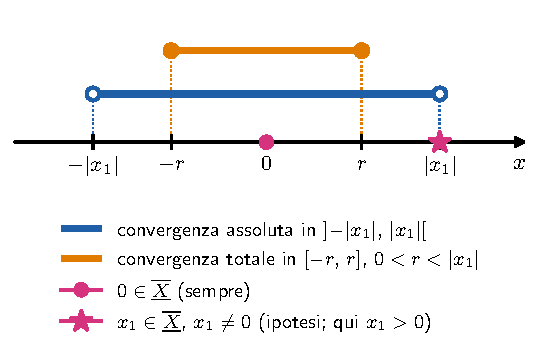
\includegraphics[width=0.8\linewidth]{figure/fig_10}\caption{Teorema~1, parte~1: se la serie converge in $x_1\neq0$ (nel disegno
$x_1>0$), converge assolutamente in $\mathopen{]}-|x_1|,|x_1|\mathclose{[}$ (in
blu) e totalmente in ogni $[-r,r]$ con $0<r<|x_1|$.}\label{fig:10}\end{figure}

\paragraph{Osservazione.}
% [0:32:52]
Per la parte~1 basta \emph{un solo} punto $x_1\neq0$ di convergenza per avere la
convergenza assoluta in tutto l'intervallo simmetrico
$\mathopen{]}-|x_1|,|x_1|\mathclose{[}$; per la convergenza totale bisogna
restringersi un po', a $[-r,r]$, come per la serie geometrica.
% [0:34:30]
Nella parte~2 non serve chiedere $x_2\neq0$: in $0$ la serie converge sempre.
La parte~2 dice che, trovato un punto di non convergenza, la serie non converge
nelle ``code'' $|x|>|x_2|$, cioè lontano da $0$.
% [0:35:48]
In particolare non serve studiare a parte i punti negativi, e $\Xconv$ potrà essere
solo $\{0\}$, un intervallo di centro $0$ oppure tutto $\mathbb{R}$: proprietà
che una serie di funzioni qualsiasi non ha.

% [0:37:02]
\paragraph{Dimostrazione della parte 1.} Sia $x_1\neq0$, $x_1\in \Xconv$: la serie
numerica $\sum_{n=0}^{\infty}a_nx_1^n$ converge.
% [0:38:26]
Deduciamo da questa ipotesi tutto ciò che si può con l'Analisi~1:
\begin{itemize}
  \item il termine generale è infinitesimo (condizione necessaria):
  \[
    a_nx_1^n\to0 ;
  \]
  \item % [0:39:53]
  una successione convergente è limitata, quindi esiste $M>0$ tale che
  \begin{equation}\tag{$*$}
    |a_nx_1^n|\le M\qquad\forall n\in\mathbb{N}.
  \end{equation}
\end{itemize}

\emph{Convergenza assoluta.} Sia $x$ con $0<|x|<|x_1|$ (in $x=0$ la convergenza
è già nota): dimostriamo che converge la serie
\[
  \sum_{n=0}^{\infty}|a_nx^n| .
\]
% [0:42:38]
L'idea è maggiorare con qualcosa che converge, usando l'unica disuguaglianza a
disposizione, $(*)$: moltiplichiamo e dividiamo per $x_1^n$ (lecito perché
$x_1\neq0$) e usiamo il fatto che il modulo del prodotto è il prodotto dei
moduli:
\begin{equation}\tag{$**$}
  |a_nx^n|=\underbrace{|a_nx_1^n|}_{\le M\text{ per }(*)}\cdot\left|\frac{x^n}{x_1^n}\right|
  \le M\left|\frac{x^n}{x_1^n}\right|=M\left(\frac{|x|}{|x_1|}\right)^{n}
  \qquad\forall n .
\end{equation}
Passando alle serie (a termini positivi, quindi il confronto si conserva):
\[
  \sum_{n=0}^{\infty}|a_nx^n|\le M\sum_{n=0}^{\infty}\left(\frac{|x|}{|x_1|}\right)^{n}.
\]
A destra c'è una serie geometrica di ragione $0<|x|/|x_1|<1$, quindi
convergente. Per il criterio del confronto la serie converge assolutamente per
ogni $x$ con $|x|<|x_1|$.
% [0:45:18]
Ecco perché la serie geometrica è stata studiata prima: qui fa da serie di
confronto.

\emph{Convergenza totale.}
% [0:46:44]
Bisogna restringersi ancora, prendendo la $x$ un po' più vicina a $0$. Sia
$0<r<|x_1|$: per $|x|\le r$ si maggiora ulteriormente la catena $(**)$:
\[
  |a_nx^n|\le M\left(\frac{|x|}{|x_1|}\right)^{n}\le M\left(\frac{r}{|x_1|}\right)^{n}=M_n
  \qquad\forall n,\ \forall x\in[-r,r].
\]
$M_n$ non dipende da $x$ e $\sum_{n=0}^{\infty}M_n$ converge, essendo una serie
geometrica di ragione $r/|x_1|<1$: la serie converge totalmente in $[-r,r]$.

\paragraph{Osservazione.}
% [0:46:44]
Perché non maggiorare subito con $|x|\le|x_1|$? Si otterrebbe $M_n=M$, e la
serie $\sum_{n=0}^{\infty}M$ diverge (le somme parziali valgono $M(n+1)$):
nessuna informazione. Serve un $r$ \emph{strettamente} minore di $|x_1|$,
% [0:49:29]
così come per la serie geometrica bisognava restare lontani da $1$.
% [0:50:51]
È il ragionamento fatto per la serie geometrica, ma senza usare somme parziali e
somma: per questo funziona per una serie qualunque.

% [0:52:58]
\paragraph{Dimostrazione della parte 2.} Sia $x_2$ un punto in cui la serie non
converge: dobbiamo dimostrare che non converge in nessun $x$ con $|x|>|x_2|$.
% [0:54:23]
Per assurdo, sia $x$ con $|x|>|x_2|$ e supponiamo che la serie converga in $x$
(figura~\ref{fig:11}). Si ha $x\neq0$, perché $|x|>|x_2|>0$ (infatti
$x_2\neq0$, dato che in $0$ la serie converge). Allora, per la parte~1
(applicata con $x$ al posto di $x_1$), la serie converge in
$\mathopen{]}-|x|,|x|\mathclose{[}$, che contiene $x_2$ perché $|x_2|<|x|$
(figura~\ref{fig:12}). Quindi la serie converge anche in $x_2$, contro
l'ipotesi: assurdo.
% [0:57:50]
Dunque la serie non converge in $x$.

\begin{figure}[htbp]\centering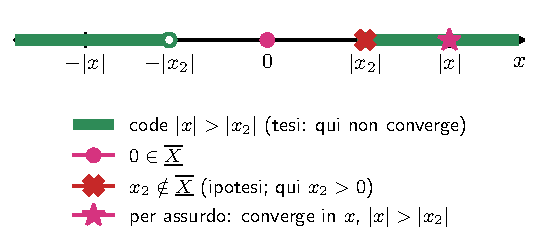
\includegraphics[width=0.8\linewidth]{figure/fig_11}\caption{Teorema~1, parte~2: $x_2$ è un punto di non convergenza (nel disegno
$x_2>0$); per assurdo si suppone che la serie converga in un punto $x$ delle
code $|x|>|x_2|$.}\label{fig:11}\end{figure}

\begin{figure}[htbp]\centering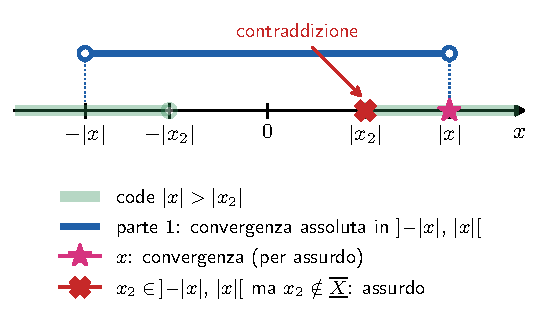
\includegraphics[width=0.8\linewidth]{figure/fig_12}\caption{Conclusione dell'assurdo: per la parte~1 la serie converge in
$\mathopen{]}-|x|,|x|\mathclose{[}$, che contiene il punto di non convergenza
$x_2$.}\label{fig:12}\end{figure}

\paragraph{Osservazione (gli estremi).}
% [0:57:50]
Se la serie converge in $x$ non è detto che converga in $-x$: all'intervallo
$\mathopen{]}-|x|,|x|\mathclose{[}$ si può aggiungere il punto $x$, ma non il
suo simmetrico. Per questo gli intervalli del Teorema~1 sono aperti. Ad esempio
$\sum_{n\ge1}x^n/n$ (vedi l'esempio svolto alla fine) converge in $x=-1$ ma non
in $x=1$: il suo insieme di convergenza è $[-1,1\mathclose{[}$.
% [0:59:19]
Da quale parte si possa chiudere l'intervallo dipende quindi dal segno del
punto, e a priori non si può chiudere.

% [1:00:05]
\subsection{Il raggio di convergenza}

Dal Teorema~1 segue il Teorema~2, che dice com'è fatto il raggio di convergenza
e quindi l'insieme di convergenza.

\paragraph{Teorema 2.} Sia $\sum_{n=0}^{\infty}a_nx^n$ una serie di potenze con
raggio di convergenza $\rho$. Allora:
\begin{enumerate}
  \item $\rho=0$ $\Longleftrightarrow$ la serie converge solo in $x=0$, cioè
  $\Xconv=\{0\}$;
  \item $\rho=+\infty$ $\Longleftrightarrow$ la serie converge assolutamente (e
  puntualmente) in tutto $\mathbb{R}$, cioè $\Xconv=\mathbb{R}$, e totalmente nei
  compatti;
  \item se $0<\rho<+\infty$, la serie converge assolutamente in
  $\mathopen{]}-\rho,\rho\mathclose{[}$, totalmente in $[-r,r]$ per ogni $r$
  con $0<r<\rho$, e non converge per $|x|>\rho$. Quindi
  \[
    \mathopen{]}-\rho,\rho\mathclose{[}\;\subseteq\; \Xconv\;\subseteq\;[-\rho,\rho] .
  \]
\end{enumerate}

\paragraph{Osservazione (il candidato insieme di convergenza).}
% [1:06:45]
Verrebbe da scrivere $\Xconv=\mathopen{]}-\rho,\rho\mathclose{[}$, ma questo è solo
il \emph{candidato} insieme di convergenza: $\rho$ è un sup e non
necessariamente un massimo, quindi a priori non sappiamo se $\pm\rho$ stiano in
$\Xconv$. Le parentesi vanno lasciate aperte, anche se nulla vieta che si chiudano.
Per stabilirlo bisogna studiare la convergenza agli estremi $x=\rho$ e
$x=-\rho$, cioè le due serie numeriche
\[
  \sum_{n=0}^{\infty}a_n\rho^n \qquad\text{e}\qquad \sum_{n=0}^{\infty}(-1)^n a_n\rho^n .
\]
% [1:08:00]
L'esercizio quindi ``raddoppia'': trovato $\rho$ si scrive subito il candidato
per $\Xconv$, ma per sapere se l'intervallo si chiude servono due serie numeriche di
Analisi~1.

\paragraph{Questioni aperte.} Restano due domande:
\begin{enumerate}
  \item come si calcola $\rho$?
  \item se l'insieme di convergenza si chiude in un estremo, cosa si può dire
  della convergenza totale e di quella uniforme?
\end{enumerate}
% [1:09:25]
Alla prima rispondono i criteri seguenti, del tutto meccanici. Alla seconda
risponderà il \emph{teorema di Abel}, che sarà solo enunciato (senza
dimostrazione) e va saputo applicare: se la serie converge in un estremo, la
convergenza uniforme arriva fino a quell'estremo; la totale, in generale, no
(vedi l'esempio svolto).

% [1:12:11]
\subsection{Criterio di Hadamard}

\paragraph{Teorema (criterio di Hadamard).} Sia $\sum_{n=0}^{\infty}a_nx^n$ una
serie di potenze. Se esiste
\[
  \lim_{n\to\infty}\sqrt[n]{|a_n|}=\ell
\]
(per la permanenza del segno $\ell\ge0$), allora
\[
  \rho=\begin{cases}
    0 & \text{se } \ell=+\infty,\\[2pt]
    +\infty & \text{se } \ell=0,\\[2pt]
    \dfrac{1}{\ell} & \text{se } 0<\ell<+\infty.
  \end{cases}
\]
Per l'algebra dei limiti (con $1/(+\infty)=0$ e $1/0^+=+\infty$) si può scrivere
in un'unica formula
\[
  \rho=\frac{1}{\ell}.
\]

\paragraph{Richiamo (criterio della radice per le serie numeriche).} Sia
$b_n\ge0$ e sia $\lim_{n\to\infty}\sqrt[n]{b_n}=\ell$. Allora:
\begin{itemize}
  \item se $\ell>1$ (anche $\ell=+\infty$), si ha $b_n>1$ definitivamente,
  quindi $b_n\not\to0$ e $\sum b_n=+\infty$;
  \item se $0\le\ell<1$, $\sum b_n$ converge;
  \item se $\ell=1$ il criterio non è conclusivo.
\end{itemize}

\paragraph{Dimostrazione.}
% [1:16:55]
Si procede come nello studio di una qualunque serie di funzioni: per ogni $x$
fissato si applicano i criteri dell'Analisi~1. È l'esercizio che si farebbe su
una serie assegnata senza conoscere il teorema; sistematizzato, diventa un
criterio. La serie non ha segno costante (la $x$ varia in tutto $\mathbb{R}$),
quindi si studia la convergenza assoluta, cioè la serie
$\sum_{n=0}^{\infty}|a_nx^n|$, con il criterio della radice (non con quello di
Hadamard, che è ciò che si sta dimostrando).
% [1:17:54]
Per $x\neq0$ (in $x=0$ c'è sempre convergenza; per $\ell=+\infty$ si avrebbe
anche la forma indeterminata $\infty\cdot0$)
\[
  \lim_{n\to\infty}\sqrt[n]{|a_nx^n|}
  =\underbrace{\lim_{n\to\infty}\sqrt[n]{|a_n|}}_{=\,\ell\text{ per ipotesi}}\cdot|x|
  =\ell\,|x| ,
\]
% [1:19:16]
perché $|x|$ non dipende da $n$ ed esce dal limite (il modulo va messo su tutto,
anche su $a_n$). Per il richiamo:
\begin{itemize}
  \item se $\ell|x|<1$, la serie converge assolutamente in $x$;
  \item se $\ell|x|>1$, allora $|a_nx^n|>1$ definitivamente: il termine
  generale non è infinitesimo e la serie \emph{non converge} in $x$ (non solo
  non converge assolutamente).\footnote{Questo passaggio non è stato esplicitato
  a lezione, dove si è mostrata solo la convergenza per $\ell|x|<1$. Senza di
  esso si otterrebbe solo $\rho\ge1/\ell$.}
\end{itemize}
% [1:20:33]
Distinguiamo i casi su $\ell$:
\begin{itemize}
  \item $\ell=+\infty$: $\ell|x|=+\infty>1$ per ogni $x\neq0$, quindi la serie
  converge solo in $0$ e $\rho=0$;
  \item $\ell=0$: $\ell|x|=0<1$ per ogni $x$, quindi la serie converge in tutto
  $\mathbb{R}$ e $\rho=+\infty$;
  \item % [1:22:02]
  $0<\ell<+\infty$: la serie converge per $|x|<1/\ell$ e non converge per
  $|x|>1/\ell$, cioè
  \[
    \mathopen{]}-\tfrac1\ell,\tfrac1\ell\mathclose{[}\;\subseteq\; \Xconv\;\subseteq\;
    \bigl[-\tfrac1\ell,\tfrac1\ell\bigr]
    \qquad\Longrightarrow\qquad \rho=\frac{1}{\ell}.
  \]
\end{itemize}
Per $|x|=1/\ell$ si ha $\ell|x|=1$ e il criterio della radice non decide: è per
questo che gli estremi vanno studiati a parte.

% [1:23:12]
\subsection{Criterio di D'Alembert}

Dal criterio rapporto-radice dell'Analisi~1 segue un altro criterio, che si
deve a d'Alembert (equivalente al precedente quando il limite del rapporto
esiste).

\paragraph{Teorema (criterio di D'Alembert).} Sia $\sum_{n=0}^{\infty}a_nx^n$
una serie di potenze con $a_n\neq0$ definitivamente. Se esiste
\[
  \lim_{n\to\infty}\left|\frac{a_{n+1}}{a_n}\right|=\ell ,
\]
allora $\rho=1/\ell$, con la stessa convenzione del criterio di Hadamard
($\rho=+\infty$ se $\ell=0$, $\rho=0$ se $\ell=+\infty$).

\paragraph{Dimostrazione.}
% [1:25:20]
Per il criterio rapporto-radice per le successioni, se il limite del rapporto
vale $\ell$, anche il limite della radice $n$-esima vale $\ell$:
\[
  \lim_{n\to\infty}\left|\frac{a_{n+1}}{a_n}\right|=\ell
  \quad\Longrightarrow\quad
  \lim_{n\to\infty}\sqrt[n]{|a_n|}=\ell ,
\]
quindi vale la tesi del criterio di Hadamard.

\paragraph{Osservazione (non dimenticare i moduli).} In entrambi i criteri il
modulo serve ad avere termini positivi, e solo in quel caso si possono
applicare i criteri della radice e del rapporto.
% [1:25:20]
Dimenticarlo non è un errore da poco: il limite potrebbe venire negativo, cosa
impossibile per un raggio.

\paragraph{Osservazione (radice o rapporto).} Il criterio della radice è più
generale: se esiste il limite del rapporto esiste anche quello della radice, ma
non viceversa. Ad esempio con
\[
  a_n=\begin{cases}1 & n\ \text{pari}\\ 2 & n\ \text{dispari}\end{cases}
  \qquad\Longrightarrow\qquad
  \left|\frac{a_{n+1}}{a_n}\right|\in\Bigl\{2,\frac12\Bigr\},
  \qquad \sqrt[n]{|a_n|}\to1
\]
il rapporto non ha limite, mentre Hadamard dà $\rho=1$. Inoltre D'Alembert non
si applica se infiniti coefficienti sono nulli: nella serie del seno, ad
esempio, compaiono solo le potenze dispari; Hadamard invece funziona
($\sqrt[n]{|a_n|}\to0$, quindi $\rho=+\infty$).
% [1:26:48]
Se non esiste nemmeno il limite della radice si usa la formula di
Cauchy--Hadamard, che vale sempre:
\[
  \frac{1}{\rho}=\limsup_{n\to\infty}\sqrt[n]{|a_n|}.
\]
Il $\limsup$ va preso sulla radice, non sul rapporto: nell'esempio sopra il
$\limsup$ del rapporto vale $2$ e darebbe $\rho=1/2$, che è sbagliato.
Calcolare $\rho$ non è quindi il vero problema: la parte delicata è capire cosa
succede agli estremi.

% [1:14:20]
\subsection{Esempio svolto}

\paragraph{Esempio.} Studiamo la serie
\[
  \sum_{n=1}^{\infty}\frac{x^n}{n}.
\]
% [1:14:20]
Prima di tutto si riconosce che è una serie di potenze: la potenza è $x^n$ e il
coefficiente è $a_n=1/n$ (la somma parte da $n=1$: manca il termine noto, cioè
$a_0=0$). Con il criterio di Hadamard:
\[
  \frac{1}{\rho}=\ell=\lim_{n\to\infty}\sqrt[n]{\left|\frac{1}{n}\right|}
  =\lim_{n\to\infty}\frac{1}{\sqrt[n]{n}}=1
  \qquad\Longrightarrow\qquad \rho=1 .
\]
Il candidato insieme di convergenza è quindi $\mathopen{]}-1,1\mathclose{[}$, in
cui la serie converge assolutamente.
% [1:15:39]
L'esercizio si riduce a un limite di successione (niente condizione necessaria
né il resto dello studio di una serie): bisogna ricordare bene i limiti di
successione.

Restano gli estremi:
\begin{itemize}
  \item $x=1$: si ottiene $\displaystyle\sum_{n=1}^{\infty}\frac{1}{n}$, la serie
  armonica, che diverge;
  \item $x=-1$: si ottiene $\displaystyle\sum_{n=1}^{\infty}\frac{(-1)^n}{n}$, la
  serie armonica a segni alterni, che converge.
\end{itemize}
Quindi
\[
  \Xconv=[-1,1\mathclose{[} .
\]
Fino all'estremo chiuso la convergenza totale non arriva: in $[-1,0]$
\[
  \sup_{x\in[-1,0]}\left|\frac{x^n}{n}\right|=\frac{1}{n}
  \qquad\text{e}\qquad \sum_{n=1}^{\infty}\frac{1}{n}=+\infty .
\]
Che arrivi almeno la convergenza uniforme lo dirà il teorema di Abel.

\paragraph{Osservazione (serie di potenze e Taylor).}
% [1:28:15]
Tutto questo non è astratto, anzi. Con i coefficienti di Taylor visti
all'inizio, il polinomio di Taylor diventa una serie (per il seno compaiono solo
le potenze dispari). Dove si dimostra che una funzione è la somma della sua
serie di Taylor, la funzione è davvero un ``polinomio infinito'', e si capisce
perché la si scriveva come il suo polinomio di Taylor ``a meno di un errore'':
al crescere del grado i polinomi di Taylor del seno approssimano il seno su
intervalli sempre più grandi, ma per avere tutto il seno serve la somma
infinita.
% [1:29:38]
La teoria delle serie di potenze spiega perché Taylor funziona. Non è però
automatico: $\ln(1+x)$ coincide con la sua serie di Taylor solo in
$\mathopen{]}-1,1]$, e la funzione $e^{-1/x^2}$ (posta uguale a $0$ in $0$) ha
serie di Taylor in $0$ identicamente nulla, pur non essendo nulla.


\end{document}
